\documentclass[12pt]{article}
%\usepackage[utf8]{inputenc}
%\documentclass[UTF8]{ctexart}
%\usepackage[UTF8, heading = false, scheme = plain]{ctex}
\usepackage{geometry}
%geometry{a4paper,scale=0.9}
\geometry{a4paper,left=1cm,right=1cm,top=1cm,bottom=2cm}
\usepackage{amsfonts}
\usepackage{color}
\usepackage{url}
%\usepackage{biblatex}
\usepackage{amsmath}
\usepackage{amssymb}
\usepackage{latexsym}
\usepackage{cite}
%\addbibresource{ref.bib}
%\bibliography{ref.bib}
\usepackage{caption}
\usepackage{graphicx, subfig}
\usepackage{float}
%\usepackage[fontset=ubuntu]{ctex}
%\usepackage{fontspec}
\usepackage{xeCJK}
%\usepackage[colorlinks,
%anchorcolor=black,
%citecolor=black]{hyperref}
%\setmainfont{SimSun}
\usepackage[section]{placeins}
\usepackage{enumitem}
\usepackage{framed}
\usepackage[framemethod=TikZ]{mdframed}
\usepackage{indentfirst}
\usepackage{setspace}%使用间距宏包
\linespread{1.5}
%\title{预备知识}
%\author{leolinuxer }
%\date{June 2020}

\title{全面解读阿里巴巴绩效体系}
%\author{leolinuxer }
%\date{June 2020}

\begin{document}
%\setlength{\parindent}{0pt}
\maketitle
\tableofcontents

\section{实事虚干——绩效管理的境界}
\subsection{关于绩效管理的四句话}
\begin{framed}
What gets dreamed,gets realized。 种瓜得瓜,种豆得豆。 

What gets measured,gets done。 所测即所得。 

What gets feedback,gets improved。给反馈才能进步。 

What gets rewarded,gets repeated。被奖励才能重复。

首先第一句话是,你做什么样的梦想,你就会得到什么样的结果,这个叫种瓜得瓜,种豆得豆,所以你要种了一个西瓜,你千万不要想, 我能收获一个芝麻,这是不可能的;第二句名言叫做,你去考核什么,衡量什么东西就会被员工所执行。第三句话,你对员工反馈什么,这个反馈的部分就会得到提升。第四个你奖励什么,这个行为就会持续的被做。这是整个绩效我认为非常经典的几个核心的话。
\end{framed}

\subsection{绩效管理的味道:实事虚干}
\begin{framed}
1. 为过程鼓掌,为结果付酬。

2. 今天最好的表现是明天最低的要求。

3. 对得起好的人,对不起不好的人。

4. 不让雷锋吃亏,向奋斗者倾斜。

5. 绩效管理是为了培养和发展员工,而不仅仅是为了考核结果。

6. 绩效管理是公司与员工的共同契约,可以双赢,也可能双输。

7. 绩效管理是点燃员工底层动力的燃料。

8. 制度保障+资源分配+游戏规则。
\end{framed}

• 我们再去理解一下一些中国企业关于绩效的一些文化和味道。第一个,为过程鼓掌为结果付费,什么意思?绩效管理当中什么是最重要的?结果,中间很辛苦,我可以说你辛苦了,但是我会给你付报酬吗?不会。

• 那么绩效管理的下一句是,今天最好的表现是明天最低的要求,这句话是阿里的经典名言。 这句话的背后是让你的绩效一天比一天做得好。

• 第三,对得起好的人,对不起不好的人,绩效奖励时应该什么公平。你应该把好的人重重地奖励,不好的人不应该奖励。

• 接下来是华为的名言叫,不让雷锋吃亏,向奋斗者倾斜。雷锋不能让他吃亏,因为华为以奋斗者为本,他们的奋斗者跟不奋斗的人,可能一年有某些部门可能奖金会差十倍。如果你的员工,你两个业务部门的老大,年底的时候一个人拿的是另外一个人的十倍,够刺激吗?你拿50万,那人拿500万,刺激吗?刺激的结果是明年我也变成下一个奋斗者。

• 下面这句话非常重要,绩效管理不仅仅是为了考评,最重要的是为了发展和培养员工。

• 绩效管理是员工和公司的共同契约,可以双赢,也可以双输。我给你做一个绩效目标,完成了咱俩就双赢,输了公司和员工双输。

• 绩效管理是点燃员工底层动力的燃料。千万不要公司想怎样,公司想怎样,如果你没有把员工开关点开,没有把动力点燃的时候,员工不飞起来,公司能飞 吗?飞不起来,因为公司由员工组成。

• 绩效管理是制度保障,是资源的再分配,也是一个公司的游戏规则,我们打游戏,王者荣耀是不是需要游戏规则的?当你公司来上班需不需要游戏规则?当然是需要这个就是我们整个绩效管理的一个味道。

\begin{framed}
老板决定什么是正确的方向,绩效管理\textcolor{red}{保障}我们走在正确的方向上

这句话是很经典的一句话,老板决定什么是正确的方向,战略就是正确的方向,绩效管理是保障我们整个公司走在正确的路上。老板说这条路是正确的,如果没有绩效保障的话,会走偏。所以绩效管理最大的作用是保障我们走在公司制定的战略的正确的路上,这是绩效保障最重要的一个作用。
\end{framed}

\subsection{企业成功=文化X战略X组织能力}
\begin{figure}[H]
    \centering
    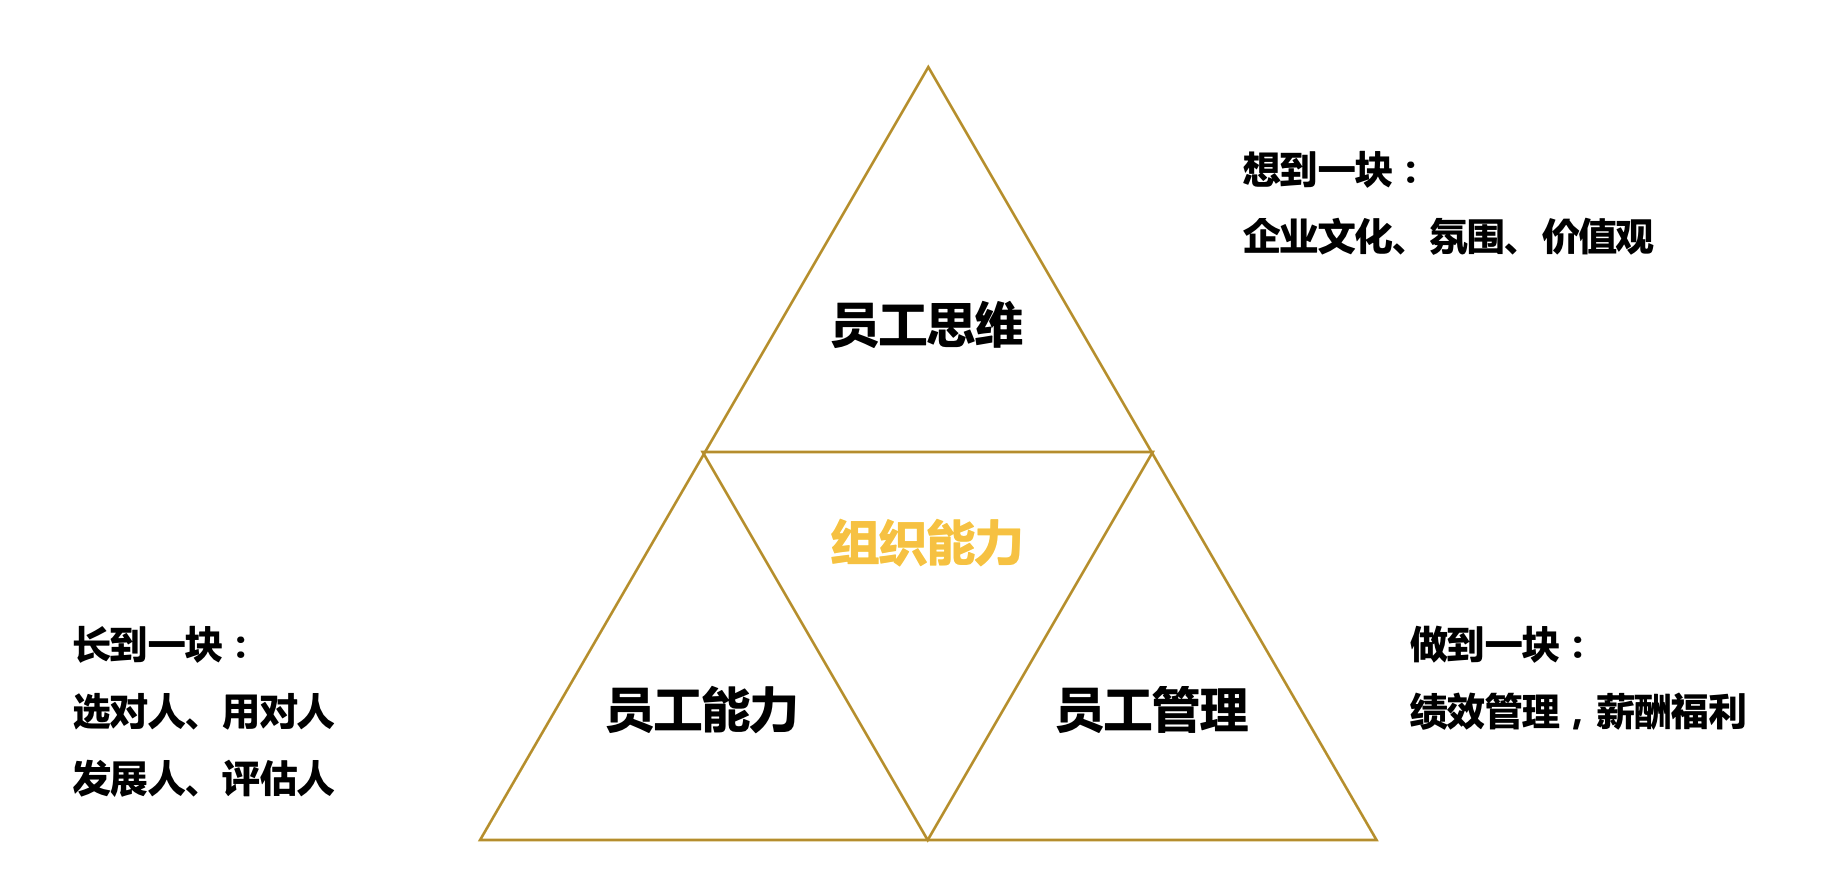
\includegraphics[width=1\textwidth]{fig/Ali_Performance_1.png}
\end{figure}

企业要跟员工真正达成双赢,是需要我们想在一起,就是企业的文化价值观和氛围,公司创造这个氛围是每个员工喜欢的。

第二个是要长到一起,我们要不断把味道一样的人招进来,还要把人用好,还要把人发展好,评估好,这就是长到一起了。 那么公司跟员工之间怎么能做在一 起,就是通过绩效的纽带连在了一起。所以只有通过文化,通过治理结构,通过我们的人员梯队建设,公司和员工才能够真正走在一起,否则它是两条平行线, 公司要什么员工说不是我要的,员工要的,公司不关注,两个永远没有办法拧成一股绳往前走,而每一个绩效的背后,真正有个好绩效的核心原因是:1. 员工愿意干这个事情;2. 员工具备干这个事情的能力。

第三,公司的所有的制度是能够激励到我的。所以这张图诠释的是公司跟员工之间怎样真正的走在一起,你是需要想到一起,思想上是需要长在一起,需要能 做到一起,所以绩效管理就承担了这部分的作用。

选对人、用对人、发展人、评估人,这就是人才培养体系。我们上面这部分,就是刚刚讲的企业文化。所以我们做管理的,做老板,都是要考虑。这 hr 课真的不是给 hr 开的,给老板开的,老板要想这些东西怎么捏在一起,我员工的心才能够跟我聚在一起,管理最难的地方是心在一起。得人心者得天下,怎么得人心, 要这么全给它揉在一起,想在一起,长在一起,做到一起。这个是很重要的,所以绩效承担的是这部分的作用。

\subsection{绩效管理的作用}
\textcolor{red}{企业的需要:组织目标达成、过程中监控各个环节}

绩效保证的是公司战略是使命愿景驱动,战略是保证我们走在正确的路上,绩效是保障我们走在正确的路上。刚才那句话是战略文化愿景使命,是让我们选择了一条正确的路。组织绩效管理是保障我们走在正确的路上。

\textcolor{red}{管理者的需要:目标分解与传递、与员工达成共识}

目标怎么分解下去,我不做绩效管理,我分不下去,我也没有办法跟员工达成共识。

\textcolor{red}{员工的需要:了解自己的绩效,上级对自己的评价,希望获得认可和成长}

员工每个人都渴望知道公司对我的评价,我该怎样反馈,我该怎样获得成长,每个人 都需要的。

\subsection{绩效管理的误区}
\begin{figure}[H]
    \centering
    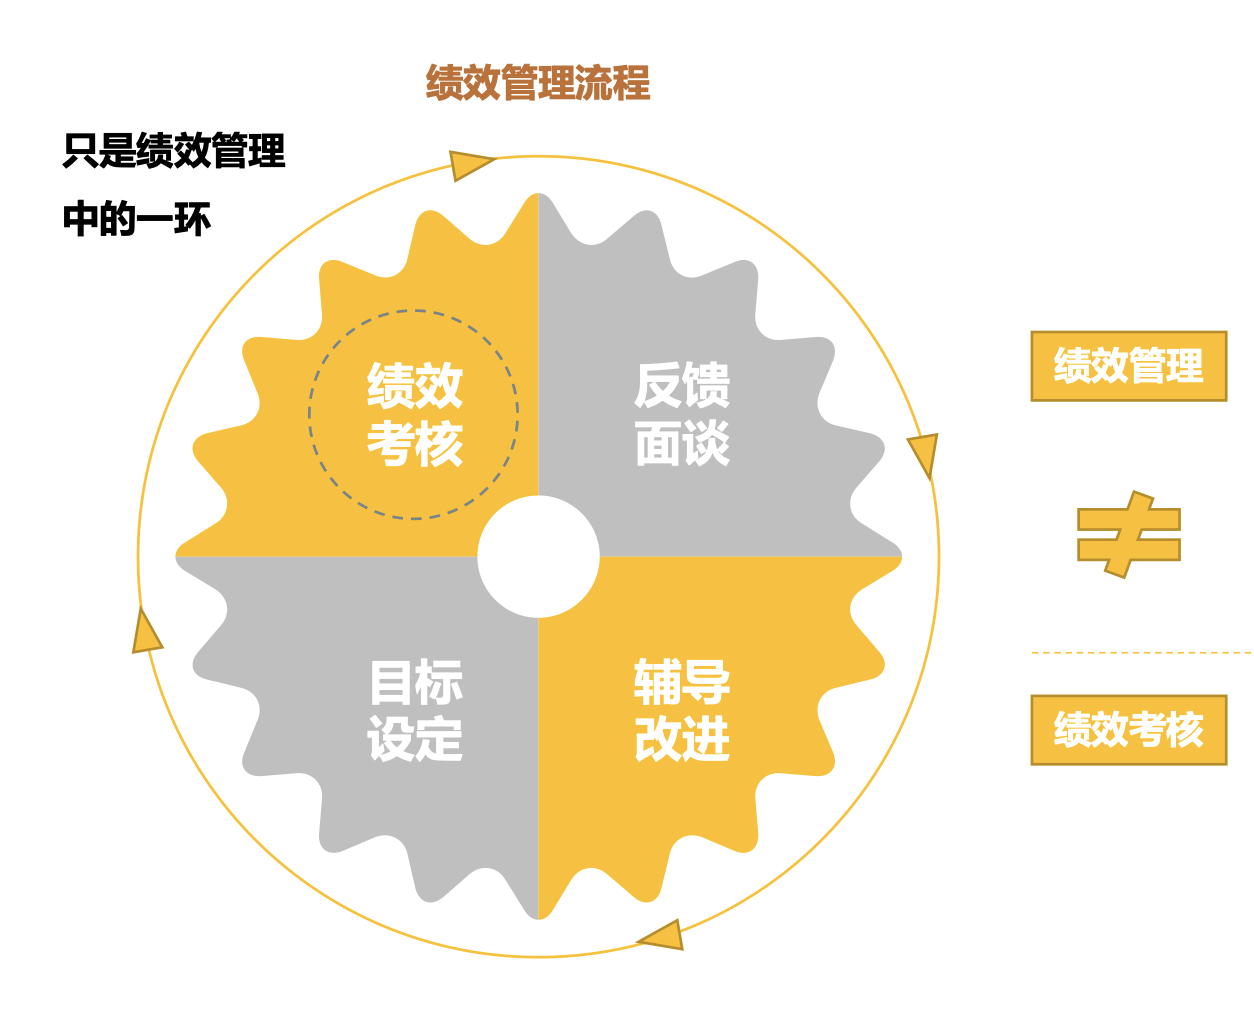
\includegraphics[width=.6\textwidth]{fig/Ali_Performance_2.png}
\end{figure}

\textcolor{red}{绩效管理不等于绩效考核}

绩效管理是:
\begin{itemize}
\setlength{\itemsep}{0pt}
\setlength{\parsep}{0pt}
\setlength{\parskip}{0pt}
    \item 为达到目标而达成共识的过程,以及增强员工成功达到目标的管理方法;
    \item 一个持续不断的交流过程,由员工和他的直接主管之间达成的共识来保证完成;
    \item 一个循环的过程,不仅强调达成绩效结果,更通过目标、辅导、评价、反馈,达成结果的过程。
\end{itemize}

绩效考核是:
\begin{itemize}
\setlength{\itemsep}{0pt}
\setlength{\parsep}{0pt}
\setlength{\parskip}{0pt}
    \item 依据既定的标准,通过一套正式的结构化制度和系统的方法,评定和测量员工工作结果。
\end{itemize}

• 绩效管理有个误区,有没有听过另外一个词叫做绩效考评。为什么阿里是从来不提绩效考评的?我们只说绩效管理,原因是绩效管理和考评之间有巨大的差异。 因为绩效管理,首先要跟员工达成共识。第二跟员工不断地去交流和辅导,最后他是通过追踪整个目标,辅导评价反馈以后,其实背后的目的是为了培养和发 展员工,这就是绩效管理的作用。

• 绩效评估的话仅仅是考评最后一个环节,绩效管理大还是绩效考评大?管理范围更大,因为它是一个周而复始,PDCA的一个过程,考评只是里面的一个环节。

• 绩效管理是整个循环,从目标的设定,然后我对你打分,然后我不断的给你反馈,面谈,不停地跟踪,我的目的是为了发展。而考核只是最后那个按钮,合格还是不合格,考核的意义大不大? 节点上是大的,但整体上是没有意义的,你考核我我不合格了,员工会觉得你这是秋后算账,为什么我不合格?你为什么不早点告诉我?为什么不早点反馈,为什么早点对我辅导?所以大家一定要明白绩效管理的是为了发展员工,而绩效考评是为了那个节点,告诉你,你合格还是不合格,优秀还是不优秀。绩效管理不等于绩效考评。

\section{绩效管理体系的设计与落地}
\subsection{绩效管理工具的分类}
\begin{itemize}
\setlength{\itemsep}{0pt}
\setlength{\parsep}{0pt}
\setlength{\parskip}{0pt}
    \item OKR (目标与关键成果法) Objectives and Key Results
    \item PBC(个人业绩承诺) Personal Business Commitment
    \item BSC(平衡记分卡) Balanced Score Card
    \item KPI(关键绩效指标) Key Performance Indicator
\end{itemize}

绩效管理工具的选择依据:根据
\begin{itemize}
\setlength{\itemsep}{0pt}
\setlength{\parsep}{0pt}
\setlength{\parskip}{0pt}
    \item 不同战略
    \item 不同业态
    \item 不同价值观
\end{itemize}

选择不同的绩效管理工具。

• 市面上有很多不同的绩效管理的方式。华为用了 PBC(个人业绩承诺),谷歌用了 OKR,大型业务单一不太变化的公司会用平衡记分卡。阿里目标导向的公司会用 KPI,绩效管理每家公司是不一样的,一定要选择一套适合的绩效管理的工具,这由由公司不同的战略,不同的业态,还有不同的文化价值观决定的。 举个例子,阿里曾经有一年引进了一个 HRVP 专门来做平衡积分卡,他是中国平衡积分卡的专家,想在整个集团内部去推行平衡计分卡。

• 但是三个月不到项目就废掉了,因为平衡积分特别适合比较单一的大型的不太变化的业务,我们是天天变,体系没建完都变了,根本就来不及。另外,平衡积分卡的习得比较困难,我们的管理者可能要学半年才能学会。马总说这不行,这东西弄完,自己就崩溃了。所以不同绩效管理方式选择的背后,还有非常核心的东西,是老板价值观的选择。

• 举个例子,同样文化大家都在说很重要,为什么只有马总把文化价值观作为50\%的考评分数,因为他知道任何事情都要矫枉过正,他心目中文化是排第一的, 所以必须以这种极端的方式。文化必须占到50\%的考核,第2他深度相信一个价值观好的人业绩一定是好的,他不认为考核价值观会阻碍业绩的发展,这是他内心的价值观选择。比如华为也很重视文化,但它所有的考核都是沿着大项目的业务考核,说明任总背后还是业务第一的。华为价值观也会落地,但并不计入考核分数,他用一个管理委员会的方式去解决这个问题。 大家都知道腾讯以产品线为考核的,说明马化腾背后的核心就是产品第一。所以你们知道不同的价值观选择的背后,核心有两条,一条是我们不同的业务要用不同的考核方式,第二,是由我的价值观决定的。

• OKR 在美国硅谷非常流行,为什么中国能够用 OKR 的特别少,因为谷歌的员工都是精英,都是自我驱动的,中国大部分的员工没有到这个程度的。如果变成 OKR 啥也不考核,打卡也不弄,肯定是不行。像 PBC 的是个人业绩承诺,一定适用于大客户业务的,所以整个项目负责人就要承担整个业务,像华为这样的 一个case 500亿 800亿的特别适合。所以绩效系统都是不同的业务和不同的价值观决定。

\subsection{绩效管理体系的建立程序}
\begin{figure}[H]
    \centering
    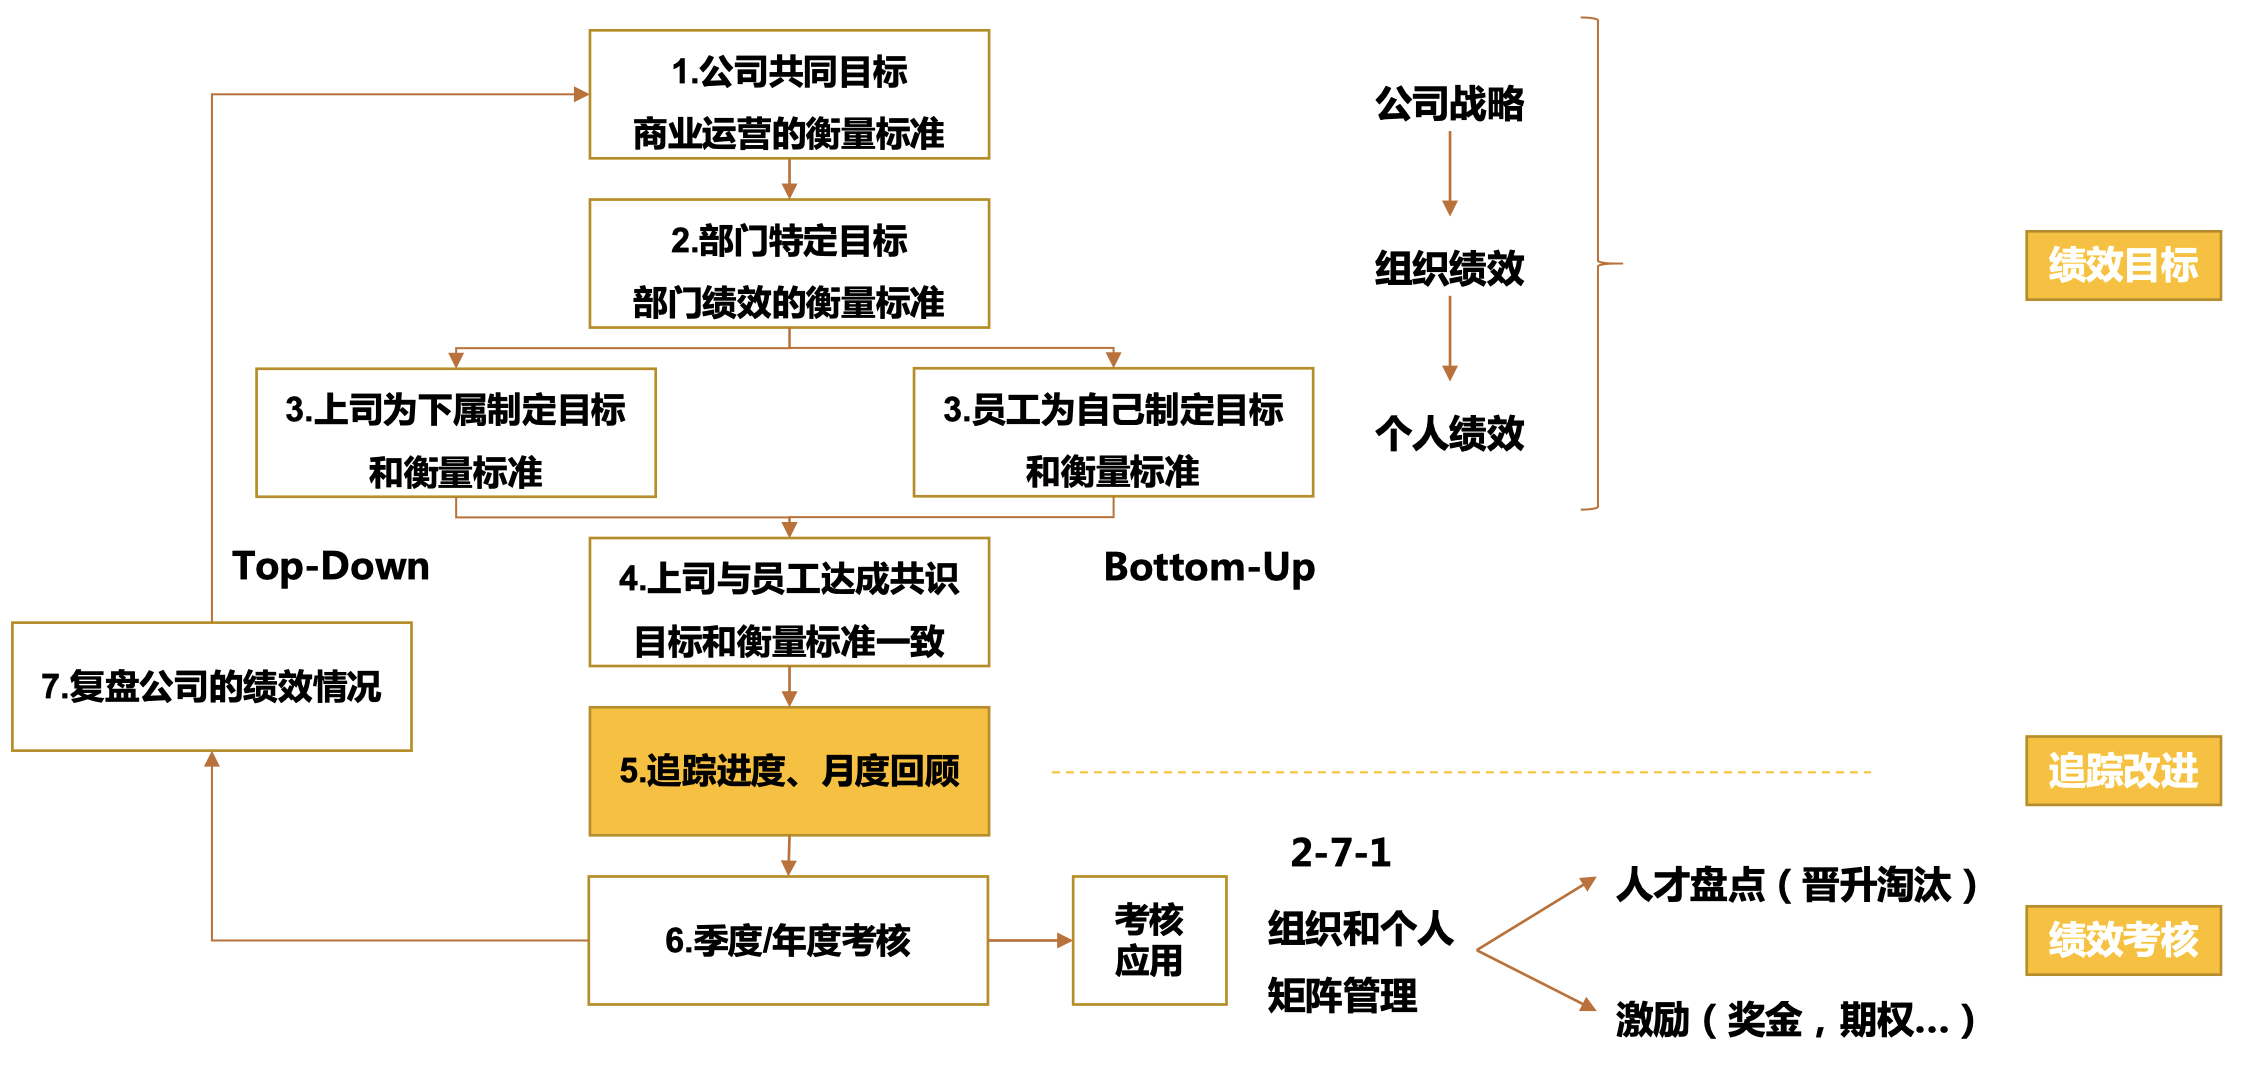
\includegraphics[width=.6\textwidth]{fig/Ali_Performance_3.png}
\end{figure}

• 建立自己的绩效的管理体系,首先公司应该有个共同的目标,大家知道的公司战略到绩效,公司的愿景、使命导出了战略以后,战略就落地到公司的商业计划书。所以第一个部分,就是目标的设置。目标设置完了,应该落到各个部门,部门下去后落到每个员工,这个时候特别重要,有两个维度,一个维度是老 板为下属制定目标,第二不要忘记员工为自己制定目标。

• 我们刚才说了文化的引擎是双向的,如果你只是一个目标给了员工,员工没有自发的想要一个目标的时候,你们俩是串不到一起去的,这个目标是你的不是我的,所以在这个地方一旦是变成个人的目标的时候特别重要,是需要经过这么两个过程的,自上而下,自下而上的融合,最后要达成一个共识。达成共识 是特别重要的第四步,否则绩效是根本落不下去的,老板的目标没有员工发自内心的认同是落不下去的。

• 那么到了这一步以后,追踪体系是非常重要,我把最重要的步骤全标黄了。

• 最终体系就是我们在目标执行落地的时候,我要每天、每周、每个月、分别用到什么机制去最终,这就是业务老大要干的事儿。追踪,改进和辅导,很重要。 那么最后通过辅导追踪以后,季度或者半年度的考评就出来了。hr在哪里?在这个目标落地的过程当中,hr的作用是什么?就是跟业务老大一起来追踪,一个追踪业务一个追踪人,就一起来配合。最后考核完了以后,我们会得出分流2-7-1人才盘点,有的人会晋升,有的人会淘汰,有的人会转岗,有的人会调离, 那么同样跟个人最相关的信息部分,奖金、晋升、未来全都出来了。所以为什么说绩效管理是每个员工底层的引擎,因为你不点燃到这一层,不跟员工的个人利益息息相关挂钩,没有用,你的引擎是点不起来的。

• 这个做完之后,要去复盘整个公司的全年度绩效考评,而且用矩阵的方式去复盘,因为那么多部门要正态分布,正态分布完了之后,再回到整个公司年初的目标去对照,这是一个完整的循环。

\subsection{绩效管理流程图}
\begin{figure}[H]
    \centering
    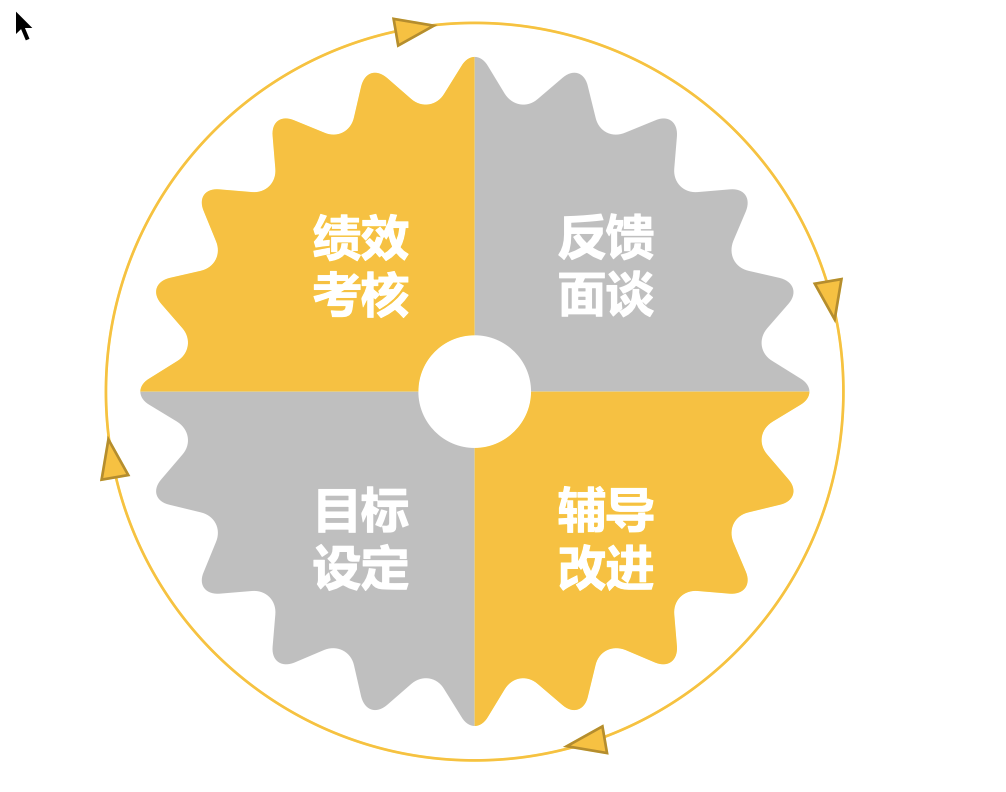
\includegraphics[width=.6\textwidth]{fig/Ali_Performance_4.png}
\end{figure}

\subsubsection{目标设定——从组织到个人}
\begin{figure}[H]
    \centering
    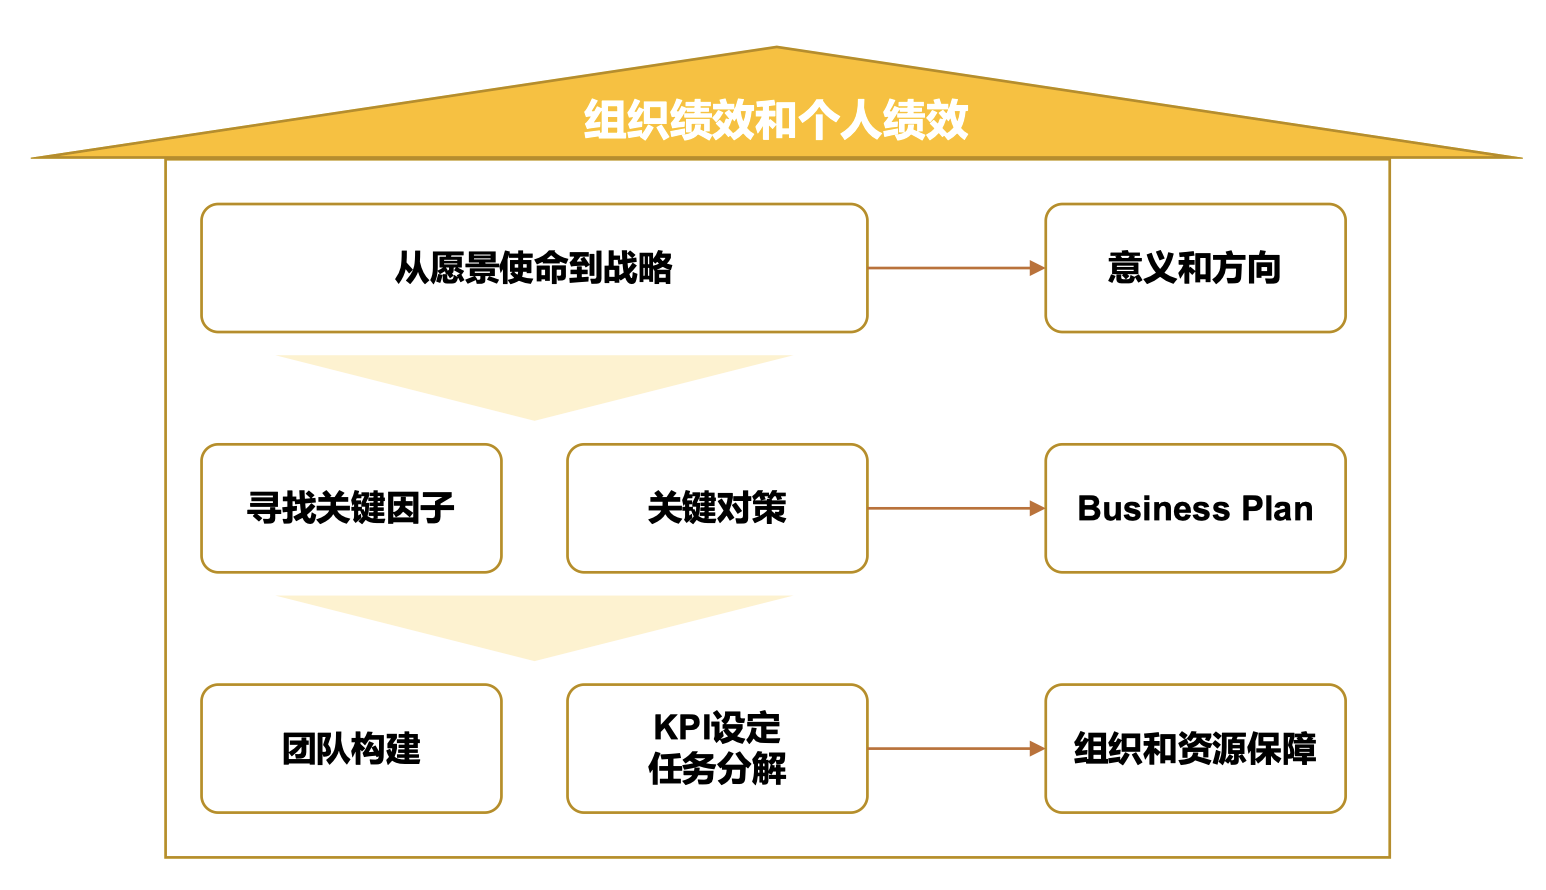
\includegraphics[width=.6\textwidth]{fig/Ali_Performance_5.png}
\end{figure}

第一个目标设置,从愿景使命价值观设立到战略,战略涉及到整个公司的 盈利目标,营运目标再层层落到部门, 再落到个人,尤其要注意落到个人的时候,一定要双向达成共识,否则是落不下去的。那么在落地的时候一定要有组织保障,组织保障就是业务老板和hr这套体系都要跟上,否则你就落不了这套制度。

\subsubsection{绩效考核}
考核不是秋后算账,目的是辅导和发展员工。

\subsubsection{反馈面谈}
\begin{itemize}
\setlength{\itemsep}{0pt}
\setlength{\parsep}{0pt}
\setlength{\parskip}{0pt}
    \item 为什么要面谈:反馈是被证明最有效的提高绩效的方法;
    \item 两种反馈阶段:日常反馈;正式Review;
    \item 三种反馈类型:正面反馈;负面反馈;建设性反馈;
\end{itemize}

\begin{framed}
面谈的基本原则:

1. 立场要坚定,今天的最好表现是明天的最低要求

2. 你是绩效管理的Owner

3. 丑话当先,永远No Surprise!!!

4. 不要轻易被不重要的事情所左右

5. 公正、真诚、善意

绩效面谈是实的事要虚干。绩效里虚的就是两个部分,一个部分是绩效管理背后的意义,第二个部分是绩效面谈,就是怎么去跟踪辅导这些员工,这个不做就一点都做不好。如果只是打分有什么意义呢?每一次绩效面谈都是最重要的辅导员工的机会,因为实践证明,反馈才是提效的方式,没有反馈是不会进步的。

第二,反馈分两个阶段,一个阶段的平常工作日常给他反馈,还有是我们一个月或者一个季度正式的反馈了。

第三,反馈包括三种,正向的反馈,负面的反馈,建设性反馈会吗?我观察到你有个问题,这个问题未来可能会比较重要,所以我给你三点建议,这叫建设性反馈。

绩效面谈是有些基本性原则,第一个老板在谈绩效的时候一定要立场坚定。 今天最好的表现是明天最低的要求,是不变的一个立场。第二,绩效管理,你是最终的主导,很重要。第三,丑话当先,永远不要有意外。最怕的绩效管理是什么?员工在进来跟你讲话之前,他觉得自己是朵花,老板今天找我,肯定有好事儿,要晋升我给我加工资?当进去的时候发现,老板说你表现不好,你可能要被调离或者降级,或者甚至要走人,这个时候员工会掀桌子就走了。因为他觉得特别意外。因为你没有提前告诉他说你哪里做的不好,你没有之前就给他一种负面的反馈和建设性意见,告诉他这里出问题了,要赶快改进。

绩效管理很重要的基本原则是不要轻易被不重要的事情所左右,你跟一个员工谈,这个员工是管理者的时候,我们看\textcolor{red}{管理者三个维度,带团队的能力,管业务的能力,自身价值观}。跟他谈什么,肯定要挑出,对他来说最重要的。比如说A管理者,他最大的问题可能是业务管理能力不行,我跟他重点反馈,B管理者什么能力都很OK,就是心胸不够宽广,所以可能是价值观的辅导。这就是辅导的重心,所以不要轻易被不重要的事情所左右。

比如说进来一查考勤,员工迟到了一次,后面再也没迟到过,然后你就拍着桌子说你为什么迟到?然后通篇都在跟他扯迟到的事情,这就是非常忌讳的事,因为你跟他复盘的时候,你是盲人摸象,你并没有抓到他的整个情况,然后把重要级给排出来。所以在谈绩效原则的时候,第一,要的是一张全貌,全部。第二个,你要跟他谈之前要排优先级。第三,每个你要跟他谈的重心可以记一下,一定要把案例放上去。 没有案例,人家是不会信服的,一定要把案例放上去,这样有理有据,人家才能够得到反馈和学习。

最后最重要的事情,每一个做绩效面谈的人,就是去评估跟员工谈话的管理者,或者hr,最重要的是永远要本着一个公正、真诚善意的态度。没有公平就没有权威,自己都不真诚不坦诚的时候,别人怎么能够放开心扉跟你聊,比如说你问他,你为什么迟到?这段时间什么不好? 员工不会告诉你说我跟我老婆离婚了。你只有很真诚的时候,他会告诉你老板,我有困难,你能不能帮帮我,所以你要足够的真诚。善意是考评的出发点,不是为了开掉他,也不是为了找小鞋给他穿,出发点是为了你好,是来帮你的。这个点一定要非常正确。我看到很多员工跟领导之间的冲突,我听他们谈话就知道,老板的出发点就不对,就是为了让员工走人,然后不停的给他挖坑,员工也不傻,他也感觉到了,这个时候他会反抗,最后就是两个人不欢而散。
\end{framed}

\begin{framed}
面谈流程

\begin{figure}[H]
    \centering
    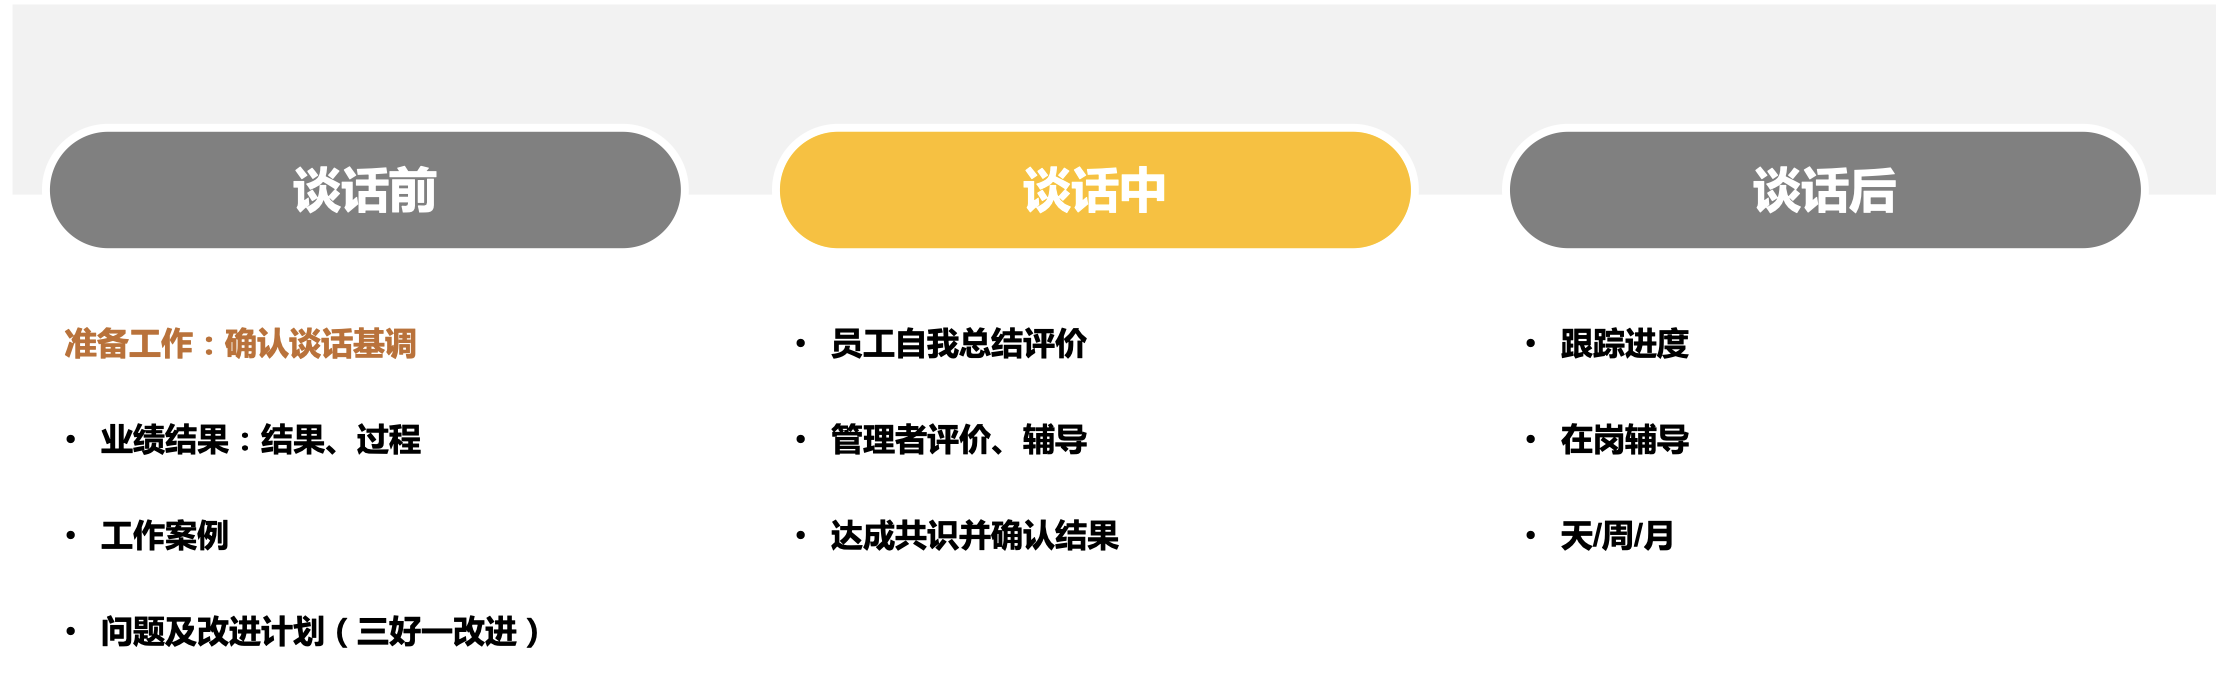
\includegraphics[width=1\textwidth]{fig/Ali_Performance_6.png}
\end{figure}

绩效面谈的流程也分谈话前、谈话中、谈话后。这个很简单,谈话前一定要充分准备好。首先跟他确认,第一我这次跟他谈话主要是为了表扬他,还是为了批评他,绩效的基调。

第二,要准备他跟业务相关所有的数据,你要分析这个员工到底是结果不好,还是过程不好,还是方法不对。

第三,你要去看他个人价值观和管团队的时候,这些问题全部都给它列下来,但是不要忘记\textcolor{red}{三好一改进},我们去批评一个人的时候,我说你123456全是缺点, 那个人会崩溃了。老板我不改了,我反正是烂泥扶不上墙,我也不想改了。所以你只有告诉他三好一改进的时候,他会有动力,你看我有优点,我就这缺点我再改改。这是沟通的非常重要的技巧。

所以在谈话中的时候,首先要开放的谈,让员工自己去评价自己。第二,我来评价你,但我更多的是以辅导的方式、引导的方式给你很多案例,最后要达成共识,要确认这个结果。管理者最大的工作在谈话以后,要根据我们达成的共识,去跟踪,在平常工作的过程中辅导,每天干嘛、 每周干嘛,每月干嘛,是有计划的,那么这样等到下个月再跟他沟通的时候,上个月跟他反馈的问题,他是不是会有改进?因为不断的强调重复的时候他就会去做,你去奖励他的时候,表扬他的时候,他就会不断的去重复的去干。所以对于管理者来讲,基本上所有的时间都是在谈话以后。

你会发现绩效管理10\%的时间是在考评,90\%时间是不在考评而在天天观察员工,辅导员工,培养员工跟员工沟通,解决他心里的疙瘩,都是管理的事情。
\end{framed}

\subsection{员工发展的理念}
提升改进,除了公司管理者要花这么多的时间以外,我们也特别提倡员工要自发自觉,,成长是你自个儿的事儿,但是公司会提供平台。
\begin{itemize}
\setlength{\itemsep}{0pt}
\setlength{\parsep}{0pt}
\setlength{\parskip}{0pt}
    \item 成长与发展是员工自己的事情,公司会提供平台。
    \item 成长与发展的机会是平等的,但机会是自己挣来的。
    \item 上课并不等于成长,成长是不断超越期望。
\end{itemize}

\subsection{绩效管理如何落地}
首先第一个部分是整个绩效管理体系的设计,体系管理的设计包括了目标 KPI的设置,包括了考核的原则,包括了考核的制度,文化怎么通过绩效考评落下去。

第二是必须要有组织保障。首先业务管理者得盯着这个目标,一直追踪。hrbp要跟着业务老大一起追踪人的发展和变化,是双向组织保障。

最后,做一次绩效管理不够,得每个季度都做循环往复做,才有可能变成一个正向的,螺旋式上升的循环,就能往前往上发展。

\subsubsection{目标及KPI设置}
1. 方向性强:突出本季/本年度重点。

2. 全面:反映员工的主要工作领域。

3. 目标具体:有明确的衡量指标,能量化的量化,不能量化的,有清晰的描述。

4. 权重设置合理:能代表员工在不同的目标的工作投入度,低于10\%几乎没用。

5. KPI设定的时间及时。

6. KPI设定不能和日常的管理工作脱节,设定要及时和员工达成共识;评估合理;日常交流和正式review的交流一致。

7. 书面描述清晰,标题:方向性明确;描述:对实现方向,有详细的工作计划或描述;对衡量有明确的说明,对3分,3.5分,4分的获得,标准清晰;顺序。

\subsubsection{KPI设置中的常见问题}
目标设置的KPI设置是有标准的,方向要强要全面,权重要适宜,要及时对等等。

KPI设置中常见的问题:滞后,一个季度过去了,刚刚开始设置。第二,找不到关键指标,什么 叫关键指标?你整个业务流程当中最重要的环节,可能没找到。 第三,过分业绩导向,忽略了团队管理和文化,那么你培养出来的人都是低分的,都是单能,只有一块能力。管理者如果没有管理团队的能力,查一下的考核,你的考核中一定没有对他团队管理能力的考核。我看过多少, KPI永远只有业绩那一条,永远没有对人的发展培养有考的,他怎么可能会长起来,因为你老板 就考核我业绩,我别的能力肯定不发展。你的管理者都不会培养人,不会带人。不会做文化,公司能发展吗? 这是你对他没有考核导致的,考核的目标极其单一,这是很重要的一个问题。

\subsubsection{组织保障}
\textcolor{red}{追踪绩效九字真言:盯目标,追过程,拿结果}。我一旦设置绩效目标和KPI,第一件做的事情是盯着,天天盯着、每周盯着、每个月盯着,第二,要去追踪这个目标,完成中间的核心环节关键指标,这叫追过程。 第三,拿结果,我要去盯他的方法,万一他的方法错的时候,就是南辕北辙的。所以一个管理者在追踪绩效落地的时候,他最重要的是要 盯目标、追过程,结果。

\textcolor{red}{追踪绩效工作方法:第一叫做情境辅导,第二叫 PDCA,第三叫16字辅导方针}(见下一章),这三个东西要同时用,辅导才会有效。我们在定目标、追过程、拿结果的时候,我们去盯的时候,你回到团队,你面对的是一个个人,个体, 每个人是处于不同的情境当中,有的人属于特别成熟,有的人属于特别不成熟,所以每个人的情境是不一样的,所以第一个你要放到情境 管理里面。然后第二,要不断的去做PDCA的循环。第三个你要做16 字辅导方针,这三个方针都是同时用,才能做得到,这是方法和工具。

\section{情境辅导—你的员工在哪个发展阶段}
\subsection{情境辅导:辅导的有效性}
1. 寻找辅导的机会(走动式管理)

2. 确认被辅导者的意愿

3. 识别被辅导者的情境

4. 十六字辅导方针

5. PDCA的不断循环(C是最重要的)

• 先讲辅导的有效性,举个例子,比如说今天要去辅导唐总,唐总心里从来不认为自己不好。你觉得你的辅导有效吗?所以你知道辅导的有效性只存在于,你看到一个人真的看不下去,你觉得这个人很烂,但是你千万要憋住气,万一那个人没有觉得自己很烂,他觉得自己是朵花,你跟他说什么他都听不进去, 这个时候辅导是没有效果的,所以选择做辅导时候,要去选择那些有辅导意愿的人,有配合度的人,你 一定要去选,觉得自己有问题,或者说我特别渴望老板你来帮帮我。然后通过你的辅导和帮助,他的结 果会好的,这叫做树榜样。

• 第一,你要寻找辅导的机会,你要看看谁有问题,并且他意识到他的问题,他愿意被你辅导,很重要。

• 第二,识别辅导者现在处于哪个阶段,就跟我们企业发展是有阶段的,每个员工它也处于不同的阶段。我们来看看员工的情境,假设一个员工,他今天刚刚坐上经理,对他来说这个工作他从来没有做过,他原来做销售的时候可能是个业务的高非常厉害的Top Sales,然后他做主管的时候可能带十个人的团队也带得特别好,他今天做了北京城市总经理,他管一百个人,这个时候总经理岗位,他是个菜鸟,他没管过。只要是这个事他没做过,他马上进入这个循环这个循环叫做员工发展的情境的一个循环。
\begin{figure}[H]
    \centering
    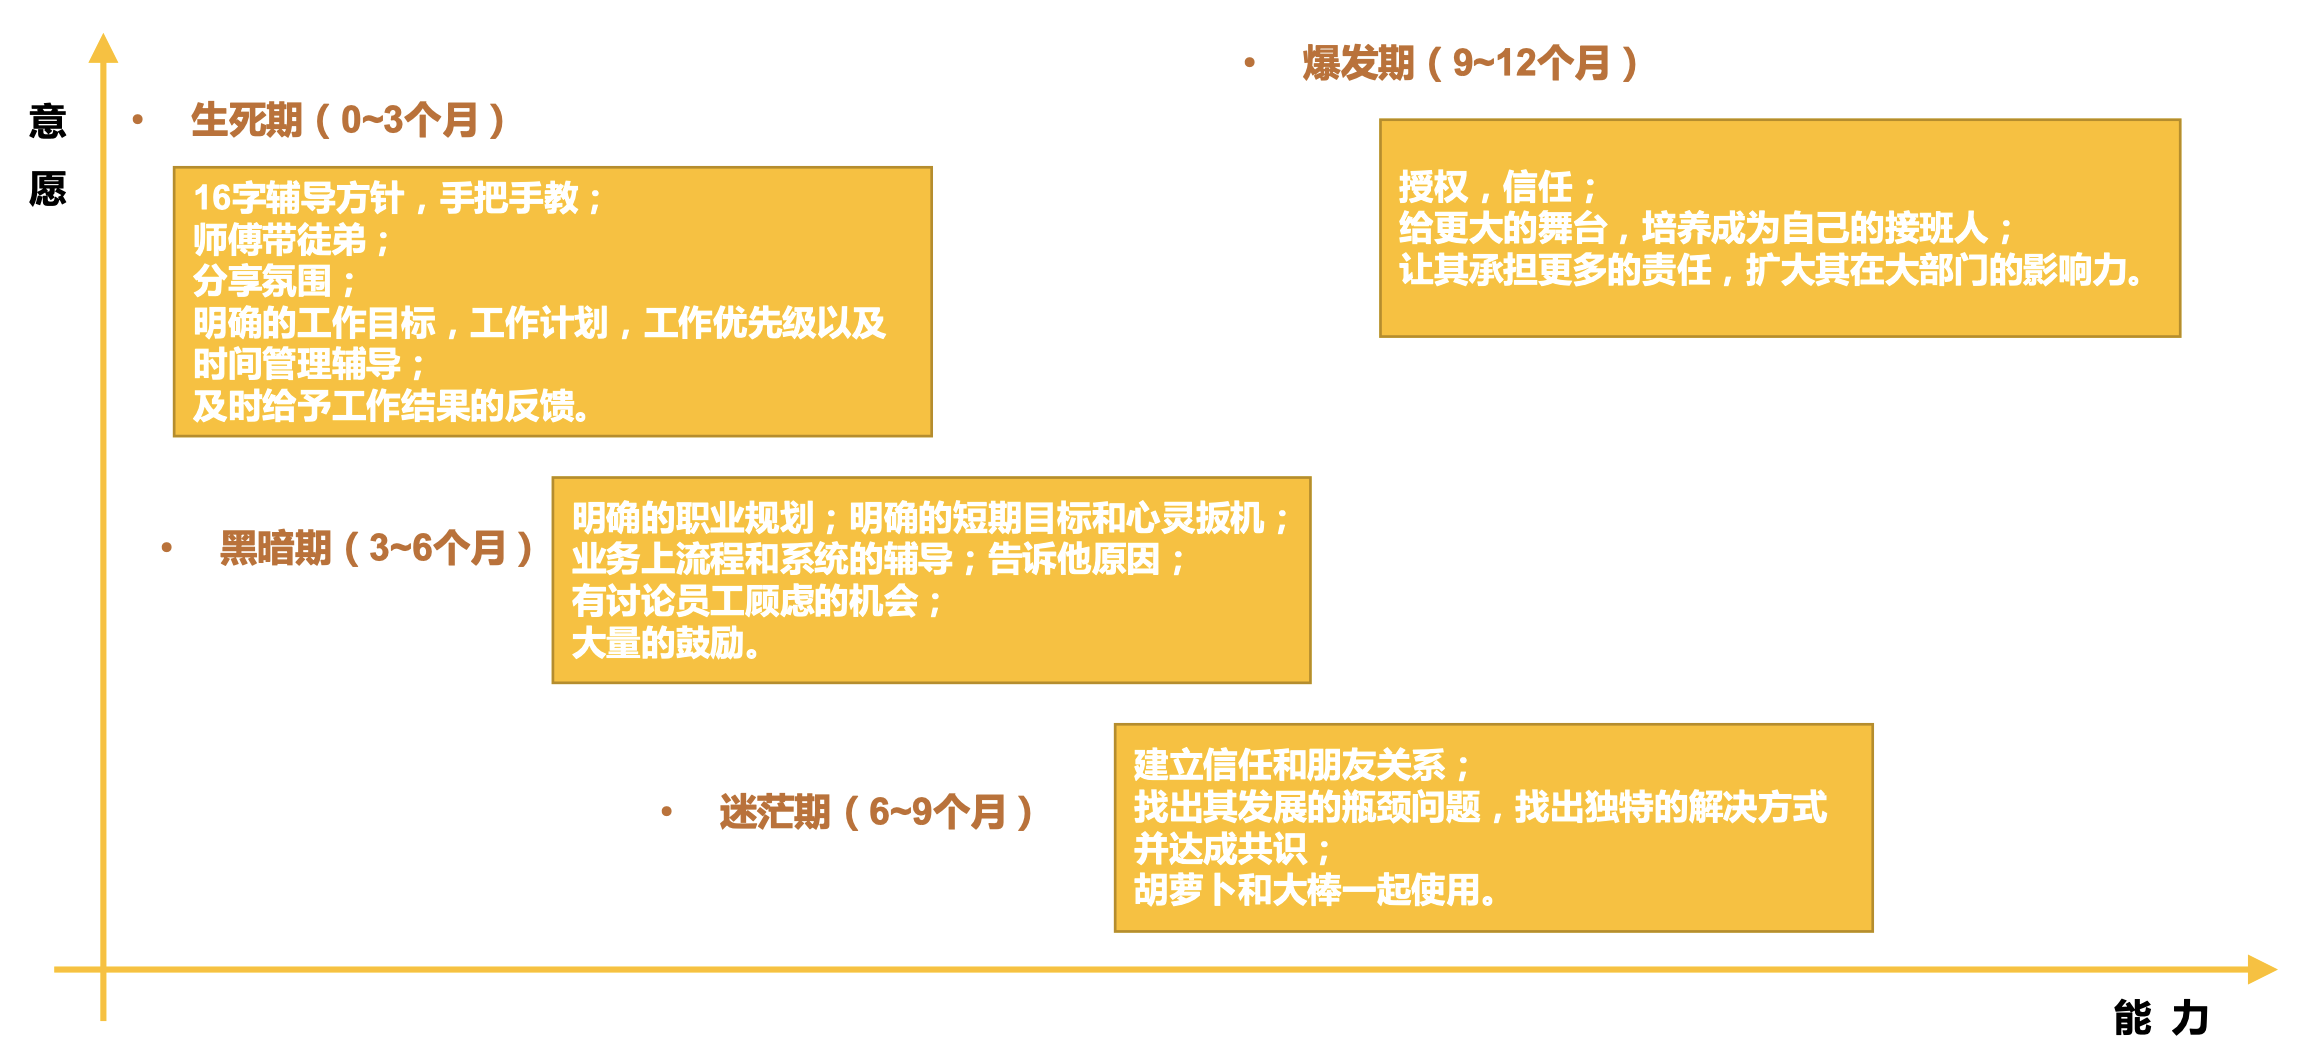
\includegraphics[width=1\textwidth]{fig/Ali_Performance_7.png}
\end{figure}

• 循环以12个月为例,纵坐标是员工有多愿意干这个事,横坐标是员工干这个事情的能力。一个刚刚当上总经理的人,在第一个阶段,他的意愿在四个阶段里是最强的。刚晋升的时候叫做新官上任三把火,特别想干出成绩来,所以这个时候意愿特别强,能力是最弱的,所以这个点员工在第一个象限,这个点应该在左上角。0到3个月往往是生死期。因为他有满腔热血又不会干,最麻烦的是乱放炮,新官上任三把火把自己给烧死。那么如果你识别员工在这个地方,这个时候他最缺的是工作的方法,所以这个时候你需要手把手的教他,方法是最重要的。

• 过了3个月以后,逐步开始适应工作环境,他的意愿热情下降了一些,因为他遇到了巨多困难。能力因为时间还是短,没有巨大的提升,所以第二个期就挺黑暗的。这个时候他最需要的是鼓励,他的意愿已经下来,另外你要把他的方法做个总结,因为他以前的方法都是点的,12345678,这个时候你要告诉他, 作为一个总经理,你一天最重要的三件事,一个礼拜最重要的三件事,一个月最重要的三件事儿是什么。告诉他体系化的知识,所以A点和B点在辅导业务的时候是不同的,A点每天告诉他123456你该干什么,B点的时候是要告诉他体系,做好总经理核心的三点,人性该怎么抓,团队该怎么带,业务体系该怎么抓,业务体系里面三条:第一条建立数据仪表盘,第二条分析你的战略和策略,第三挑,定目标追过程拿结果,然后工作习惯,开始辅导体系了。

• 到6到9个月的时候,工作经验强起来了,处于迷茫期,他的意愿是最弱的。 所以这个时候要告诉他,我一定是会支持你的,他有个瓶颈,你要给他找出来, 再加油,就走出这个循环了。

• 员工走完最后一个阶段就很光明,到了爆发期,到Q4的时候一个聪明的人用心的人,他就找到了方法,然后拿到了结果,这个时候他的状态就变成了最高。 刚刚做这个事的时候,是纯粹的激动,咱们开始当官了,这个时候他找到了这个事情的成就感,包括他能驾驭这个事情是发自内心的真正的高意愿。他的意愿是最高的,能力也是最强的,这个时候要给他更高的目标,给他更高的舞台。

• 所以最优秀的员工基本上一年都会晋升,因为他完成了循环,有的人是两年做完有,三年做完,一般来说最优秀的一年做完。所以管理系统的工具第一个就是情境辅导,你要知道你的员工到底在哪里,在哪个阶段,才能抓到重心。你如果对一个已经到了爆发期的员工,还天天跟大家讲方法,他肯定不想要这个, 我想知道我明年干嘛,我想看看我这个经验能不能到全国去推广,要的东西是不一样的。

\subsection{十六字辅导方针}
\begin{framed}
事:我做你看,我说你听,你做我看,你说我听

人:晓之以理,动之以情,诱之以利,绳之以法
\end{framed}
• 辅导的有效性。我们让员工学会的一件事,永远是通过这16个辅导方针,做事情上面:我做你看,我说你听,你做我看,你说我听。这16个辅导方针,就是 学习路径。举个非常简单的例子,一个新员工要学会如何做电话销售,第一件事情他希望老板跟他讲道理,还是说老板先打个电话给我听一下?你要培养个 Top Sales去见客户,他希望老板说你不要怕,还是带你去一遍。所以辅导的第一件事永远是我做你看,第二件事,我来跟你讲讲道理,为什么我这么干,第 三个事,我们做管理的人最大的错误就是,我说你听以后认为辅导已经结束了,他不再关心说你做一遍给我看,你再总结一遍给我听。所以我们经常会跟员 工讲,我都跟你说十遍了,为什么你还不会,好累,你怎么这么笨。背后的原因是因为你没有让他做,你没有看,你没有让他去做总结。

• 对人的辅导也是这样的,晓之以理,你要先以真情去打动她,又跟他讲道理,然后又告诉他好处,如果他不行,还得绳之以法。所以这个也是对一个员工的 辅导的流程。

• 最后PDCA告诉大家,在所有的盯目标、追过程、拿结果中最重要的,P是plan计划,D就是do,C就是check,A是action,在所有的追踪过程当中,C是 最重要的。没有追踪就永远不会拿到你要的结果,所以追踪是我们所有的过程当中最需要花时间的。

\subsection{HRBP在绩效管理中的角色和行动}
四要
\begin{itemize}
\setlength{\itemsep}{0pt}
\setlength{\parsep}{0pt}
\setlength{\parskip}{0pt}
    \item 清楚团队的目标和方向;
    \item 要善于观察并立即行动;
    \item 熟悉公司的制度和业务;
    \item 以身作则;
\end{itemize}

四不要
\begin{itemize}
\setlength{\itemsep}{0pt}
\setlength{\parsep}{0pt}
\setlength{\parskip}{0pt}
    \item 不要传递错误信息;
    \item 不要幸存侥幸心理或者胆怯;
    \item 不要逃避责任;
    \item 不要没有变化;
\end{itemize}

• 最重要的是组织原则。One over One plus HR 一个员工在公司中最重要的生命周期,无非就是他在公司中的几个重要的事情,第1入职,第2转正,第3晋 升,第4可能是转岗,第5可能是淘汰。这些重要的环节都是一个员工在一个公司里面最重要的生命周期。在这个周期里面,如果hr都不参与的话,有没有起 到价值?我们hr跟业务的分工,业务是盯人那条线,hr这条线其实也是管理者要盯的,只是你太忙了,我再帮你盯一盯。所以最后的意见都是两个人结合在 一起,只有老板和hr连在一起,这个事情才能做的好。所以在HR在这里头角色和定位特别重要,所有在员工的重要的节点中,一定要参与。

• 做的最好的公司,hr是有一票否决权的,比如,招聘中老板说这个人要招,我面完了,我是hr,我说 这个人不能招。当我们意见不一致,谁也说服不了谁的时候,否决权在哪里?在HR。一个特别好的公 司,一定是hr具有战略地位,并且跟老板是在工作职能上是三权分立的,还有财务。没有做到三权分 立,凡是一切以老板为中心的公司,都是不太具备组织能力的。从结构设计上都是有缺陷的,这叫结 构性缺陷和系统性风险。 所以hr需要做一些事儿和不做一些事情。

• 最后一条,绩效管理是一个循环的过程。Q1做完了,持续跟踪到Q2,直到QX一直在跟踪,背后就是 所有人的能力,通通的通过绩效管理,年复一年,日复一日地发展了。

\section{如何辅导“挑战权威型”业务骨干}
\subsection{辅导案例之一}
第一个案例是我做主管的时候,人生第一次做管理者,我有了十个最基层的下属,到现在为止印象很深刻,是有个员工叫桃花,这个员工是顶尖的销售Top Sales,但这个人桀骜不驯。她怎么签单的?跟客户就是背诗。她原来是艺术系的,学表演、导演的,后来又做DJ,声音特别好听。她到我部门来以后永远都 是全国二、三名。她每天就唱歌,跟客户背诗,然后订单哗啦哗啦就来了,我们销售想跟学习,发现学得会吗?学不会。第2,她特别傲气,别人跟她说话她也懒得理。我作为她的主管跟她讲,她也不理我的。 她当时的业绩非常好,但不是个明星,因为她的价值观距离公司的还是挺遥远的。这个员工技能很高, 但是她的工作意愿不可琢磨。她也不服从领导和分配,这样的员工应该怎么去鼓励呢?

事实上这个员工真的太有个性了,智商比你还高,怎么办?后来我就想了个办法。我当时有十个员工,我就把它分成271了,在培养什么样的员工变成明星的时候,是老板最能出权威的?一定是那种执行力很强的,看上去不是那么聪明的。所以我当时就选了两个案例,两个案例都是执行力特别强的,很愿意上进很勤奋的小孩,但真的是不聪明,在桃花眼里这两个人她是绝对看不上的。我就花了三个月时间把这两个小孩给拔起来了,一下业绩一飞冲天。

在这三个月当中,我对桃花进行了冷处理,你有事你找我,我回答你,没事我坚决不找你。3个月以后,她自尊心特强,她突然发现那两个小孩,突然超过她了,她受不了了。有一天走过来跟我说,老板,我受不了了,你怎么这么不爱我?一点都不关注。我说我哪里不关注你了,她说你看你光管他们不管我,我说那是因为你不要我管嫌烦,她说那我请你吃个饭,咱俩就算抹清了,你管我呗,就这样。从那以后我们就成为了一辈子的朋友,她生活中的困难,都会来跟你说。那个时候是我做管理的第一个阶段,我记得她是最难管的一个员工。

第二个员工也很奇葩,我们也是此生的好朋友,作为一个管理者还是很有成就感。这个小姑娘也是业绩非常棒,非常要求上进,家庭条件也挺差,但非常漂 亮。她怎么签单的?那个时候根本没有视频,我们是电话销售。她弄一个视频架在自己的电脑上,跟客户聊聊天的时候,化个口红就把单子给签了,也是非 常神奇的一个姑娘。这个姑娘的前任老板跟我讲,这个姑娘就是心性不太稳定,但是资质实在是太好了。后来我第一次见到她的时候,我就跟她聊天,发现 这个姑娘最大的困境是在于说她的恋爱观,因为她家里太困难了,所以她找男朋友的时候永远是把钱放在第一位。

你说她真的贪钱,也不是,她就是那种底层特别缺乏安全感,他们家全部都是靠她的,所 以他找了几个男朋友,全是以钱为出发点的,结果每次都失败的特别惨。 我就跟她聊了很 久,后来她说老板,我下次找男朋友,你帮我看看,我说好的。所以她现在的老公就是我 帮她挑的。从她感情稳定以后,这个女人就一飞冲天,后来做到了主管做到了经理,后来做到了一家公司的 hr head,她一辈子都很感谢。其实我也没帮她什么,就是帮她处理了这 个问题,老板对员工的辅导重要不重要?但是辅导的东西,\textbf{首先第一个,你要确定他有没有被你辅导的意愿。第二个你要排出员工的优先级,很多时候优先级不一定是业绩}。

\subsection{辅导案例之二}
我再给大家举第二个案例,是我刚刚做区域经理的时候,我接了一个老经理的班,这个经理下面有三个主管,三个主管里面一个主管特别老,老主管在全国 50个主管里面排名第三,你想他是不是很骄傲。第二个主管是一个中主管,做了差不多半年左右,还不到一年的时间,业绩在全国差不多排二三十名。那么 第三个主管是刚刚晋升的主管,什么都不会,刚刚晋升上来的主管,满脸热情,但是不会干,就这三个主管。

我在去接这个部门之前,前任经理是非常老的,99年到工到阿里巴巴,相当于创始人那一批,个人威信很高。我去的时候,这三个人在老主管的带领下给了我个下马威。他们集体跑到当时的副总裁那边,去告诉他说我们集体抵制一个新的经理来管我们,因为我们的老经理很厉害, 我们听说新经理是不行的,而且刚刚上任管不了我们,所以我们集体抵制我去上任。厉害不厉害?厉害,进去之后我想肯定要单个击破,我就跟他们都聊了聊。

老主管极其不配合,他觉得为什么这个经理应该是我不是你,你凭什么?他永远是不配合的。 第二个经理是摇摆的,这个姑娘其实我发现她的资质特别好,而且对自我的要求特别高。小的主管确实资质也没那么好,刚刚起步,也没什么基础,属于懵懵懂懂的,所以他也不会那么强烈的去反对你。这就是三个主管的情况。请问大家怎么在三个月之内摆平这三个主管?

\textbf{你看这些员工处于什么阶段? 从中主管下手,因为她最具拉升的潜力,她又是不上不下的那种,因为老主管的话你很难解决他的思想问题,新主管的话,解决了他的问题, 也不会有那么明显的提升,所以展现不了领导能力,拿不到阶段性成果,所以要从中主管下属}。我就是这么处理的,就因为老主管天天跟你唱反调,所以你知道为什么我给你们总结的\textbf{辅导的第一条是先确认对方愿意被你辅导},要记住对方不愿意被你辅导,是绝对无效的,所以那个主管我根本就不理你。你爱找我找我,不爱找,我不找你。你的团队我也不管,你管。

我在未来的三个月把所有的时间都花在了中间那个主管,我告诉她,我们定个阶段性目标,我来帮助你,三个月之内从25名变到前3名。 她说我跟你玩,那我有要求, 1234我都给她提了最高的要求。我说你们团队只要做到了,我也会不断的去扶植大家,所以她们整个团队我也是经常在大会上去表扬,她有成绩的时候。第三个组,就是最新的主管组,我也给他设了一个目标,我说现在你是新主管,排名49名。我说我给你一个目标三个月,你做到全公司的15名以内,他说我跟你玩,但我说因为你什么都不会,所以回到第一个象限,你都听我的,每天我告诉你怎么做,然后你早上我们来过工作计划,晚上我们复盘一遍工作计划做的怎么样,管得非常紧,而且他所有的会议 我都去参加,因为我要手把手地去辅导他就是16字辅导方针,每天就带在身边管。

然后三个月以后结果出来了,就是我们的中间主管变成了全公司第2名,然后我们最下面这个主管变成了全公司第8名。然后很遗憾,我们的老主管原来是第3名的,他掉到了整个公司第15名,这个时候老主管压力特别大,你知道他的压力来自于他的团队。他的团队说老板我们怎么回事,我们部门怎么掉的那么低。为什么新老板好像不喜欢我们,天天喜欢别的组,我觉得我们这样没有前途,他觉得有点扛不住压力,他也很好胜的,后来来找我摊牌了。他说老板,我觉得你不公平,罗里吧嗦一大堆,这个时候他来认怂的时候,是你一个辅导的机会。我说一个人再厉害,也得低调,第二,我说你作为老主管,其实你应该去帮助新主管,你有很多地方做的是不够的,我就开始跟他辅导,我说你认不认?他是我认的,我说你信不信任我?他说我看你把这么多小的都搞起来,我觉得我资质比他们好,所以我也认你,那行,我说我也给你定个计划,但我在未来三个月给他定的计划全是他在价值观层面的改进计划,不仅仅是业务上,因为他业务上已经炉火纯青了。

后来我们最辉煌的时候,六个月以后,我待的部门从0到6个月,我们的三个主管全部都进入了全公司前五名,一个是第一名,一个是第三名,一个是第四名。六个月后, 所以我们部门就是一下变成了全国第六个月的时间。所以情境管理重要不重要?如果说你没有把员工放在不同的情境里面,其实你的方法是不对的。

\subsection{辅导案例之三}
难度升级。我去广东负责整个广东省的时候,整个广东省是全国最差的,当时跟浙江的用户数一年差几万个。广东的第二个恶劣的现象,每一天都有人办离职, 因为业绩不好,大家都没钱赚,所有人都要离职。第三,广东团队没有任何管理者,理论上来说,你作为广东的负责人,下面应该有经理,经理下面应该有主 管,完全没有管理者,你的下属都没有进入到第一个象限。

在这么一个严酷的情况下,怎么用一年的时间把它翻牌,老板就是给你六个月。这个情况是我遇到过最恶劣的情况,也是我职业生涯中最辛苦的一段时间,我在广东每天三班倒,8点钟到晚上6点,第一班,8点到12点,第二班,2点到3点,第三班。那个时候压力大到晚上要看佛书才能睡得着。我相信每个人都有那段时间,人一辈子可能最大的回忆就是你最苦的那段日子。广东是我最苦的那段日子,因为情况最恶劣。

简单讲讲广东我是怎么整的,我去之前,因为浙江省做得最好,在浙江省里面所有的主管大老板也支持我,说你去谈一遍,谁愿意跟你去广东你去谈,给他优惠政策,告诉他优先晋升。我就拿着尚方宝剑跟所有杭州的主管全去谈了一遍,有人愿意跟我走吗?就一个。为什么?做管理的人永远是按照业绩的收入提成的,浙江省是最好的,在这儿第一,不辛苦,下面的人都很成熟,第二,不用背井离乡。第三,今年稳稳当当那么多钱,是算得出来的。如果跟我去广东的话, 背井离乡,肯定都是最差。那个时候,全国倒数10名的sales,广东占了8个。所以他完全没有必要,所以我在杭州的时候所有人都说我要跟着你混,我们那个圈里头都是认我。 但是真的让他们去广东的时候,这就是人性,没人去。最后有一个人,我迄今为止都非常感谢,他叫陈飞,是个典型的杭州人,一个男孩子。 他说老板我跟你去,然后我们俩单枪匹马一人一个箱子就下了广东,我这辈子也没去过广东。

在飞机上我就跟陈飞讲,这么恶劣的环境,咱们俩自己先兴奋一下。陈飞说我们定个目标,定一年能不能回杭州的目标,老板很苛刻的,做不好就回不去的。 我说我们俩总不能客死广东,很惨的,然后我说我们定个目标,我说我们12个月的时候,我们整个广东做到全国第一,有没有信心?他说老板真没信心,但是我知道没有退路,也就只能这样我们能够光荣地返回到杭州。他说现在晋不晋升也不知道,反正关键是我们能回得去。所以我们就在飞机上定了,第一, 我们12月底的时候必须要回到杭州,因为他是杭州人。

第二件事,我说我们两个到一个陌生的地方,我们总得先找点归属感了。我说陈飞,我说马上拿张地图,咱下飞机去找一个特别好的地方吃饭,然后把广东美好的东西全部享受一遍。然后我要找到对这个城市的感觉,你知道一个人去一个陌生的城市,最害怕的是你对这个城市是没有感觉的,根本待不住,天天想家。所以当时炳胜什么那些好的酒店都被我们圈出来,说一个礼拜去吃一个,因为吃在广东,要找到在广东的乐趣。后来我们又去研究广东人,我们刚好是过年过完春节,我说广东人喜欢吉利,我说俩这样,我俩明天去上班的时候,我们俩早点去,就在门口迎接,每个员工我们俩给他们包红包,获得员工的第一次好感,甭管他们现在多烂,他们得先接受你,不能把我们俩扫地出门对吧?。 所以我们下飞机后就去买红包吃东西,然后去摸点办公室在哪里,就是这样开始。所以这是我的第一个阶段。

到了第二个阶段之后,\textbf{全公司都没有任何管理者怎么办?大胆使用是最好的培养}。我跟陈飞说没办法,咱俩就只能是下猛药,公司所有的员工咱俩都谈一遍, 我们按照谁意愿最高,最想干好谁最勤奋,相对聪明一点,我们全拔出来。然后我们俩就这一个礼拜啥事也没干,就把员工一个全部都聊了一遍,最后拔了四个人。这四个人都是我们认为没有任何管理经验,但是工作意愿好,非常勤奋,很质朴很愿意上进的小孩。拔出来,我说今天你们就是代理组长,然后我告诉你做得好,三个月以后就晋升,因为公司本来是12个月晋升,但因为我是破格晋升的,我帮你们申请特殊,我说你们干不干? 他们说干,然后我就告诉他们怎么干怎么干。然后从那天开始我早也带他们,晚也带他们,每天就这么搞,搞三个月,终于基本上搞明白了这个事儿怎么做,然后他们就晋升为第一批管理者,这是我做的第二个事儿。

第三个事情是因为公司实在没人,我就招聘。那个时候招聘到什么疯狂的程度,就每天都在招聘,每一周我都去那边摆招聘摊子,每个礼拜周末全部在摆摊招聘。每一天你都在办公室里招聘。所以你知道招团队到底是hr的事情,还是老板的事情,我们那时候还没hr,全部都是我自己带着,管理者就在那里招, 然后我们给他们做招聘的表格,面试的培训,销售的北斗七星怎么化成面试表格,然后我们自己怎么练,然后你怎么初试,你怎么复试,你考核什么,我考核什么,我们自己训练,就这样。

所以在这个公司里面,前三个月我们完成了人员的一个储备,把好的人拔出来,把新的人补充进去。 0到3个月,3到6个月的时候是最黑暗的,因为我给他们压力太大了,他们基础太薄了,我基本上每天晚上都是在给他们做培训,做管理培训,很多人撑不住了,很多事,老板太苦了,我真的不想干了。那个时候北广东他们原来是特别放松的,早上9点半10点喝完早茶来上班,晚上7点钟走,在3到6个月的时候,他们没有人12点钟时间下班的,很多人就辞职了,还有人去举报,说你这个人特别不人性,这么恶搞。 你觉得我们有办法吗?这么一个环境下什么办法都没有。

到6到9个月的时候,我们开始取得了一些成绩,大家开始逐步有了一些信心,包括我们公司最差的那些全国倒数十名里头八个,终于有三个被我弄走了,另外五个人搞起来了,然后就往前跑了,大家开始有些信心了。到最后一个季度的时候,我就给他们制定了一个战役,就是一定要把杭州给他干过去。所以我们终于在11月底的时候,还没到12月,我们做到了全国第一。所以我们在12月份的时候,不仅我们俩回去了,整个广东全部回到了杭州,所有的sales我全部带回到杭州去了。 完成了杭州和广东两个省的一个合并工作。所以这是真实发生的06年的事情。

\begin{framed}
情境管理是不是很有用?刚才我的这三个案例,我作为主管、作为经理、 作为大区的时候,我自己亲身发力的三个事情跟大家诠释一下。情境就是你要去辅导一个团队,辅导一个人,一定要先把它放进去,放在那个情境里头,然后判断什么样的方式最合适的。
\end{framed}

\section{阿里巴巴六脉神剑考核解读(上)}
\begin{framed}
文化的力量摧枯拉朽,能够占领整个市场、打赢竞争对手、打造顶尖公司。
\end{framed}

\subsection{阿里巴巴的案例}
文化落地的时候,在很多公司是不考核的,我就选了一个比较特殊的案例,阿里巴巴的价值观是要考核的,就是这样,刚好把考核和文化落在一起。考核的背后选择,考核什么和不考核什么,其实背后是老板价值观的选择,为什么阿里一定是坚定不移地要考核价值观,是因为老马就信。老马充分相信, 像毛主席一样的,打土豪分田地,星星之火可以燎原,他坚信文化的力量是可以打下全天下的。 他相信文化的力量是摧枯拉朽的,能够让你占领整个市场,能够打赢竞争对手,能够把公司变成最优秀的,所以他特别极端,把价值观变成了50\%的考核。但事实上这么多年的证明,我们用大数据统计发现价值观好的员工总是高绩效员工,而相反那些价值观不太好的员工总是绩效不是很好,所以我们发现其实这条路没有走错。

大家千万不要轻易模仿,为什么这几年市面上很多的企业在模仿阿里巴巴的价值观考核落地,没有坚持三个月以上全失败了。 失败的原因是什么?第1,老板根本不信这个东西。第2,他不知道落地该怎么做,他就觉得阿里巴巴有几条价值观考核, 我就写几条价值观去考核就行了,但我们发现价值观考核落地的时候,除了有土壤以外,应该有一整套的设计理念、考核体系,并且应该由业务部的老板和hr配合, 一直追踪拿到结果,还需要不断循环往复,每个季度都要做一次,天天讲,日日讲,月月讲。如果做不到这些,不要把价值观作为一个考核,只要做一个参考就可以了。

这个案例虽然有点极端,但是我觉得非常具有代表性,不要去参考50\%,30\%这都没有关系。我们主要是去用价值观这个例子,落到绩效考评当中,怎么样算是一个比较完整好的绩效考评体系。前提和误区我都说清楚了。

\subsection{考核理念与原则}
\textbf{业绩与价值观各占50\%}:假设你今天是阿里巴巴的员工或者管理者,阿里要给你培训这套东西,你是总监,要告诉你绩效管理该怎么做,比如说我是hr, 我来给你培训,第1,我会告诉你所有员工的打分,一条纵轴是他的绩效表现,一条调纵轴是他的价值观,这两个各占50分。总分100分。这是我们设计一个总的理念。

\textbf{KPI的设定及达成共识}:在价值观打分当中,KPI的设置必须要达成共识。我们在设置绩效目标的时候,包括绩效目标中的关键指标,必须要员工和老板达成共识。

\textbf{打分的合理分布}:一般来说,一个部门里面会分271。有个组织原则,我们比较相信说10个人里头有两个是优秀的,7个是平庸的,1个是不太好的,所以这就叫271原则。所以我们会对2的员工,高绩效员工会进行奖励,奖金,晋升,一系列的激励的制度。 那么对“1”员工我们会进行强制性淘汰。在阿里硬性淘汰从来就更高,我们也是10\%,但注意10\%适合于任何一个level。我们的高管流动率也是这么高的,这个是很可怕的事情。什么叫做正态分布?比如我这个部门10个人,2个是优秀的,7个是平均的,1个是末位的,那么我这个部门是不是到时我还要集中到我整个大部门,大部门要集合到整个公司, 然后是分公司和集团一层一层往上的时候,是要重新调整比例的。你是A部门、我是B部门,但是你的绩效表现是比我好,你有两个优秀,我有两个优秀, 但最后的话就变成了你部门三个优秀,可能我一个。有可能原来我一个“1”,你一个“1”,结果变成两个“1”都是我的,你没有“1”。这个叫矩阵排布,为了公平。因为每个部门之间,横向部门其实绩效表现是不一样的。

\textbf{面谈的认真与正式}:在整个绩效管理当中,其实绩效面谈和后期的跟踪辅导环节最重要,所以这个是非常严肃的。

\textbf{跟进计划的毫不放松}:这也是我们的组织原则。

\textbf{1 over 1 plus HR的原则}:举个例子,A是B的下属,B是C的下属。我是一个hr,什么叫做one over one plus hr。我要考评A的时候,最后任命生效是什么生效方式?首先A要自评,我这个季 度,比如说100分里面得80分,但最终决定的是什么呢?第2个“one”是他的直接老板,就是B 同学,还有老板的老板C同学,然后还要加上HR共同来评定。为什么?我们的绩效面谈是one over one plus hr一去都要参与的。因为老板,直接老板很多时候会有一些偏差,老板的老板会 看得更高一点。同时如果我是你的老板,你在辅导下属的时候,你是主谈的,我是你的老板,我 是在旁边的,我的目的主要是看你有没有问题,我们叫一级辅导一级。为什么hr一定要参与?因 为hr是比较公正的,万一你们串通好了,要把下属给祸害了,hr得承担公平的角色。第2,hr会 补你很多盲区,因为你在日常管理中,基本上眼睛里业务的事情还是比较多,所以你对人的时候 很多时候会忽视掉的。我是hr,我就会给你提供很多信息。我说你对下属要好一点,最近他身体 不太好,会给你补充很多信息的,这个时候在跟下属谈的时候,你一开始就会直接问他结果好不 好,你还是会先关心他最近身体怎么样?你只有跟员工有了共情以后,员工才会打开去谈他的东 西,是不是?所以hr是很重要的。 我们最后的考评生效以后,最后一定是one over one plus hr, 全部同意打分以后,打分才会在人力资源系统里。一定要这三方全部谈过以后,绩效才算是确认, 确认以后按照绩效给你发放奖金,或者提报晋升,所以这是非常正式的一个组织原则。

\textbf{更重要的是:公正、真诚与善意}。

\subsection{阿里巴巴考核设计说明}
所以在整个绩效设计里的第一最重要的是,对绩效设计的一个理念,有了理念以后,我们要看看是第二个到底考核的制度是怎么样。
\begin{enumerate}
\setlength{\itemsep}{0pt}
\setlength{\parsep}{0pt}
\setlength{\parskip}{0pt}
    \item 员工自评要以事实为依据。员工自评的时候必须以事实为依据,你得讲为什 么是这样。我们的分数是总分5分,1分是最差的, 刻度是0.5。
    \item 通过原则。1分到5分,什么叫通关,游戏有没有打过?过不了第1关,没有第2关。通关的原则是如果你1分都没有,你就不可能有2分。因为我们会把1分当做员工最基层的东西,人人都应该做到的。
    \item 每季度考评一次。先用员工自评,然后部门主管和经理进行他评。 他评之后,one over one plus hr预约员工时间,正式开始绩效面谈,谈完之后要跟员工达成共识。
    \item 评分结果。优秀是27~30,良好是26分以内,合格22分,不合格18分。 价值观占到50\%,所以价值观得分不合格的人,就没有办法参与业务评估了,相当于一票否决权、奖金全都没有。
\end{enumerate}

\subsection{考核制度}
一、考核说明

1.员工自评或主管/经理考评必须以事实为依据,说明具体的实例;

2.如果不能达到1分标准,允许以0分表示;小数点后可以出现0.5分;

3.通关原则,之后达到较低分数的标准之后,才能得到更高的分数,必须对价值观表达从低到高逐项判断;

4.如果被评估员工某项分数为0分、0.5分或者达到4分(含)以上,经理必须注明事由。

二、考核周期及程序

1.每季度考评一次,其中价值观考核部分占员工综合考评分的50%;

2.员工先按照30条价值考核细则进行自评,再由部门主管/经理进行评价,One+One+HR;

3.部门主管/经理将员工自评分与被评分进行对照,与员工进行绩效面谈,肯定好的工作表现,指出不足,指明改进方向。

三、评分结果等级说明 1.优秀 27~30分;2.良好 23~26分;3.合格 19~23分; 4.不合格 0~18分;

四、价值观评分结果的运用

1.价值观得分为不合格者,无资格参与绩效评定,奖金全部扣除;

2.任意一项价值观得分在1分以下,无资格参与绩效评定,奖金全额扣除。

\subsection{案例:销售团队老大考核指标}
\begin{figure}[H]
    \centering
    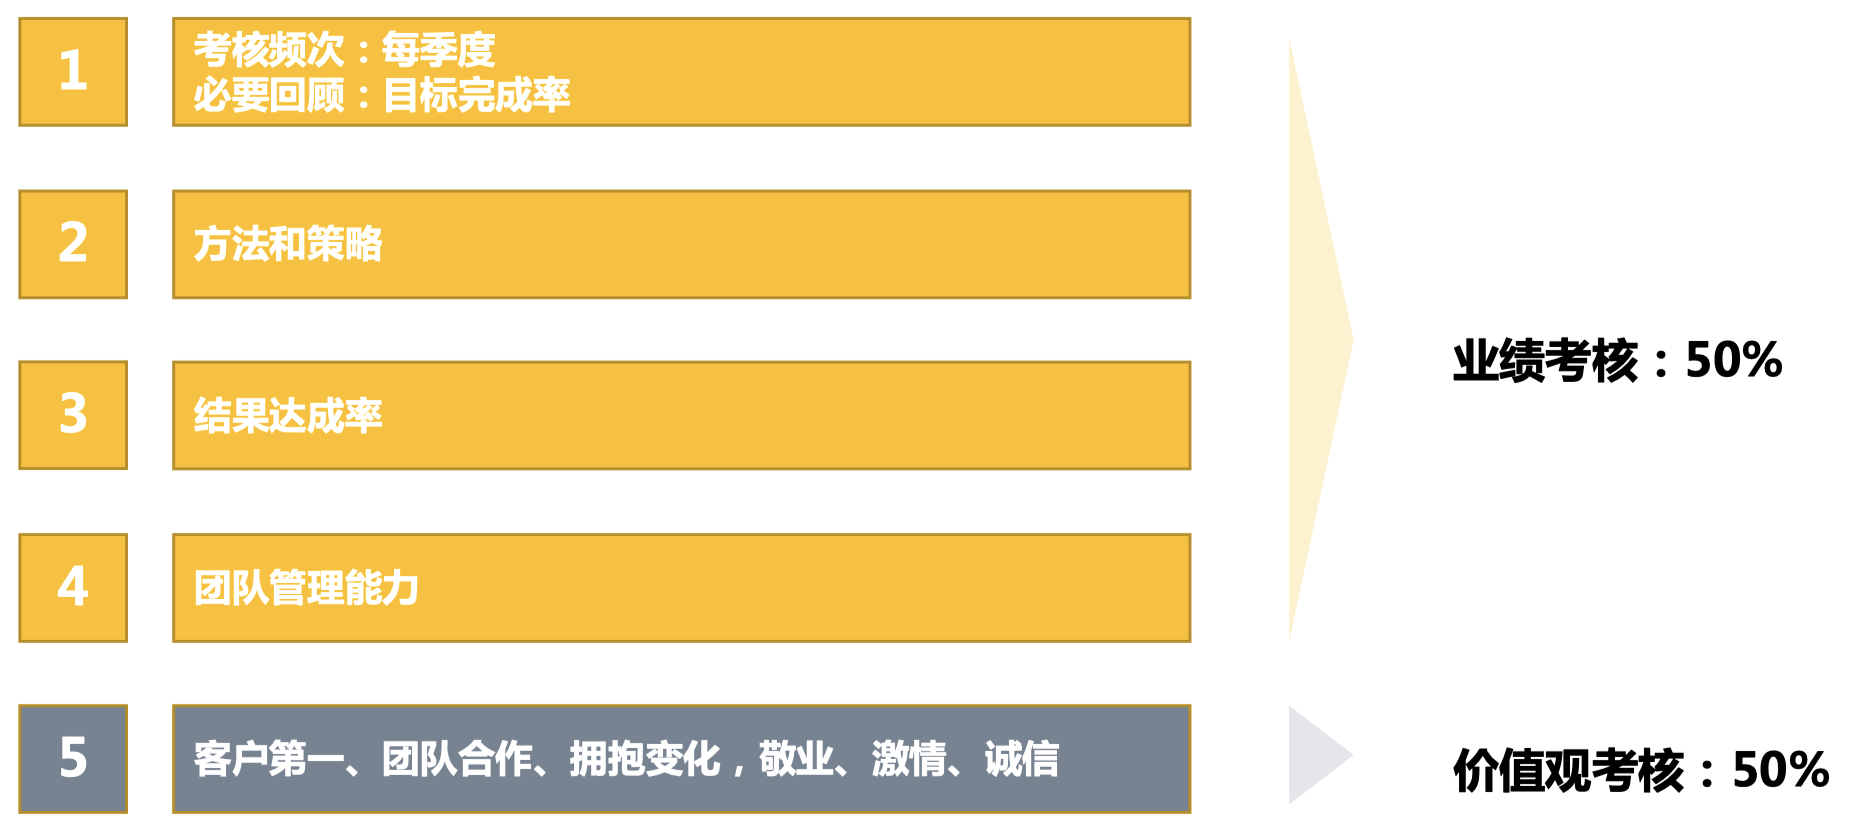
\includegraphics[width=1\textwidth]{fig/Ali_Performance_8.png}
\end{figure}

我们拿销售团队的老大的考核指标给大家看一下,我们的考核频次是一个季度打一次分。必要的回顾是,一个业务团队老大需要有目标的完成率,第 2,我们考核他的方法和策略对不对,第3,我们考核他的结果有没有达成,第4,我们考核他的团队管理能力,这全部都是要考的,那么这部分就是 50\%他的业绩部分的考核。

我们认为一个好的业务管理者,他必须是业务也很好,团队能力也很好。业务很好,包括你有没有很 好制定,科学制定目标,你的方法对不,结果有没有达成,这都是业务考核的核心,包括你的团队管 的好不好,所以4项是一共占到了50分。另外价值观占到了50分,所以就按照两部分去打分,看看总 共能得几分。我们最基础的管理者,M1——主管,3个月考核一次。经理级以上,我们是每半年打一 次分数,就每半年统计一次完整的考评,所以经理上就是半年度考核。

\subsection{评分标准}
\begin{figure}[H]
    \centering
    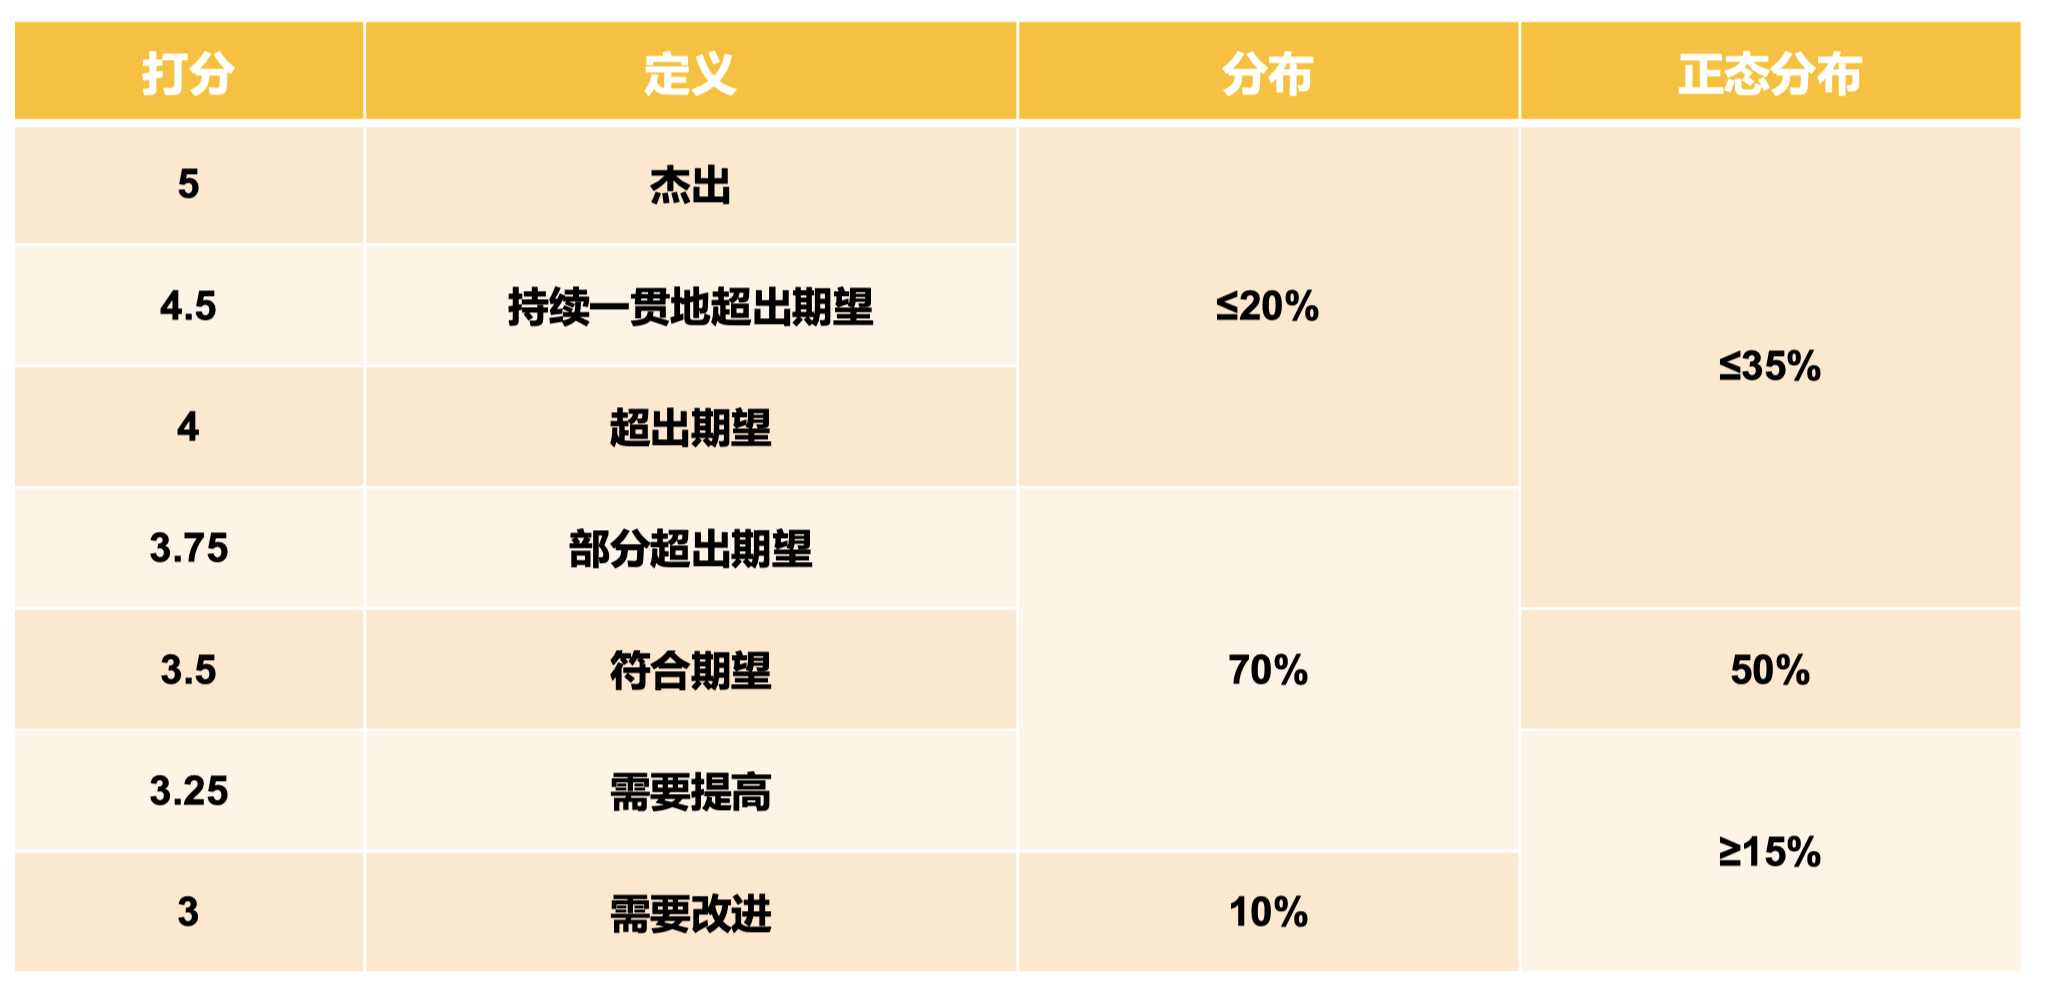
\includegraphics[width=1\textwidth]{fig/Ali_Performance_9.png}
\end{figure}
我们的评分标准是,我们有5分,每一个行为有5分,总共是以价值观为例, 公司总共是50分,另外业绩也是占到了50分。最后打分是这么一个标准, 比如3,我们认就需要改进的,肯定不太好。3分以下基本上全部就淘汰了,

3.25分需要改进。那么3.5分是满足期望,3.75分叫部分超出期望,4分叫超出期望,4.5 ,持续一贯超出期望,5分是杰出。

迄今为止,我在阿里工作这么多年,我就只被打过一次4分。我打出去4分的基本上也没有。所以你会发现,我们手是捏得非常紧的,超出期望的很少。在我们心目中优秀绝大部分就在3.75分,就是部分超出我的期望。然后3.5分基本上就是满足期望,3.25分要告诉他哪些地方你需要改进的, 到3分要给他下个严重的绩效警告,如果你不改进,下个季度有可能会被 淘汰,3分以下,基本上就直接淘汰了。基本上这是打分的情况。

正态分布是讲的是 271,10个人里面2个优秀,7个平均,1个比较弱。正态分布为什么是35、50和15?举个例子,我如果是法务部门,我这个部 门总共只有6个人,我有没有办法实行271的考核?因为我没到10个人,最小单位没到,那不可能说这6个人不给他发奖金,不给他发工资,我还是要做271的考核,那6个人乘以20\%的话是1.2个,1.2个你怎么办?老板就会去调,如果说整个部门业绩不错的话,可能1.2个人,就变成2个优秀的人了,那2个优秀的人除以6个人,它的占比就超过20\%了。所以有可能在头部的时候会超过20\%的占比,因为每个部门的情况会略有不同。比如销售部门,一般来说后台淘汰率会有10\%,但销售部门淘汰率都会更高。 很多销售部门甚至达到了30\%的淘汰率。这时正态分布,就是销售部门和技术部门和产品部门统统叠加在一起,不要高于15\%。所以这就是我们的正态分布,每个部门加起来,最后会做一个平均处理,去调整比率。

\subsection{绩效打分}
one over one plus hr打分,三个人基本上是商量好了,然后再跟员工去谈,无非是要跟员工达成共识。比如说我是你的上司,我会旁听,然后他是 hr,她在旁边旁听,然后我们都会补充,你讲完你主讲,当我们都会补充下属的情况,hr可能从人员上面补充,我可能从别的维度上去补充,所以我们正式的季度或者半年度的面谈是有这么多人一起参与的。

在3个人面谈之前,是可以先看到员工的自评表。你会发现自评的时候,从人性上来说,员工一般自 己打分高,肯定自己评自己是朵花。所以我们看到员工比如给自己打了4分。那么我们为什么面谈的时候要让他自己一条条来说案例,他只要说的出来。为什么我们这三个人要跟他谈,之前我们得先开个会,因为我们得定个调,我们到底给他评多少分。我们也是有案例的,比如说这条他没有达到,我们认为应该扣分,我们全都是逐条对过的,然后我们三个人形成共识,我们给他只能打3.5分,但他给自己打了4分。4分在阿里是一定要晋升的,3.75分有可能给你加工资,我不一定要给你晋升。这个太重要了,所以我们可能会打3.5,这个是我们在面谈沟通之前,我们三个人就得去想,怎么跟下属在沟通的时候达成共识,让他意识到不足的地方,然后让他知道他没有那么好。

\subsection{绩效面谈要达成一致}
绩效面谈,是考验员工还是考验老板?考验老板,考验老板平时关不关注员工,如果这个员工你平时根本不关注,你根本不知道他任何行为的时候,你跟他面谈的时候你会产生意见不一致,冲突,你根本解决不了,然后员工就掀桌子去了,根本不会鸟你。而且阿里,很可怕的是只要员工不确认这个分数,你们不达成共识,是没有办法走下去的。 你压力多大?你上面老板一直在催你,还不递交,你不递交我整个部门没有分数的。上级搞不定下属,下属就是不签。

当然,员工真不签的很少。所以这就是为什么你在员工的辅导前期,\textbf{你的管理要做在前面}。以前我在阿里有个习惯,我做管理的时候,我笔记本前面记录的全部都是我今天做什么事,业务上的事,反面记的全是我所有下属的案例,我今天跟他共事,我有什么事儿,我会把它记下来。 当然这不是为了秋后算账, 因为反馈要及时,如果今天只是个小事,我马上就给他反馈掉了,但如果这样的事情特别多,已经变成一个很重要的问题,我会打个大圈圈,这个问题要变成绩效谈话,让他意识到重要性,我就会把这个在他的面谈当中深入下。然后这个地方我会对他扣分。

举个例子,比如说我自己带的一个小姑娘,是一个小朋友,到我们公司来。这个小孩子我跟她去拜访客户的时候,第1次我跟他去拜访董事长的时候,她迟到半个小时,我到了,董事长到了,你们觉得这个事儿重要不重要?重要,所以我回头我回去的时候,我就提醒她,我说你下次不可以迟到。 好,第2次的时候我们又去拜访一个董事长,就在对面公司她又迟到了,你知道迟到总有100个理由,不迟到是没有理由的,然后这个时候我又提醒她了。这个时候我告诉她说,你不要超过三次,我其实是平时就提醒她了,我说你下次不要再迟到,我已经反馈给她,我并不是秋后算账。但是我在绩效考评的时候,客户第一这条价值观我会不会给她扣分?因为她不是一次,另外这个太重要了。

\subsection{绩效面谈要达成一致}
有个员工,她见客户的时候,她老喜欢穿露胸露背、露胳膊露腿的衣服,更可怕的是我们去地产公司拜访大集团老总,董事长,她也是这么穿裙子,人家董事长就快差点吓晕过去。 第1次跟她讲了,第2次她还是这样,第3次还是这样,要不要扣分?要扣分,所以绩效考评是要抓重点的。我不能说因为员工迟到1 次,而且迟到可能就是内部的1个迟到,就揪着不放,提醒你就可以了。外部客户可能更重要了。但如果持续这样,这个事已经特别影响公司的整个品牌,你认为很重要的时候,要拎出来,要扣分。所以在商量给员工打分的时候,我们就会一条条对,非常重要。\textbf{跟员工谈话的时候,没有这些案例,员工肯定不服}。

再举个案例,我们在管区域的时候,广东省下面花都有个区域经理,原来那个区域经理下面有个主管,当地有个小hr。我是当时广东省负责人,花都区的区域经理因为一些原因被公司辞退了。下面这个主管他想经理的位置肯定是我,花都没有其他人了,而且我在花都呆的时间最长,这个区域刚成立,我就在这个地方了,没有功劳也有苦劳,晋升理所应当。HR对他也挺好,当地的hr总觉得他很有前途,所以他沾沾自喜。这个时候省里头大hr跟我搭配,我们到花都, 因为这个区域经理被辞掉,这个事情是要处理的。我们下去之后那天晚上主管请大家吃饭特别高兴,不停的让我们喝酒, 他以为你无事不登三宝,下来肯定是要晋升他。因为他不是直接归我管,他还有一个大区经理在上面,我就走了。第2天早上,大区经理和大hr就跟他聊天了,就是绩效谈话。员工是带着老板今天给我晋升的心情来的。结果大区域经理和hr进去之后,他们跟他谈的是,我们其实是不晋升你。这个人很多地方是达不到区域经理要求,尤其在个人价值观和带团队的能力上面很薄弱,做业务是蛮好的,所以他其实是不合格的。所以老板跟他谈的目的是,这个地方你必须要提升,如果这个地方你不提升的话,是没有办法到区域经理的。其实我是为了你好,我想好好跟你讲,但是员工听完这个之后,10分钟之内就翻脸,把桌子都掀了,老子不干了,就走了。

这个案例充分说明了员工的期望值和管理者的期望值是有很大的差异的。后来我就批评大区经理,差异的根源在于,你没有丑话当先。员工觉得我是朵花, 今天你就要晋升我,那你早干嘛去了,你早就发现他的缺点,你为什么不是在前几次面谈的时候跟他讲,你这个地方不行,你赶快改是有问题的。所以\textbf{管理永远是事前管理,no surprise管理,最害怕是今天出现惊吓。管理既不要惊喜也不要惊吓,两个惊都不要,惊喜也是我失控,惊吓也是我失控}。

\subsection{如何科学制定目标}
\subsubsection{解决部门目标和个人目标的关系}
对管理者来说,头上有个目标摆着的,最难的是怎么把这个目标分解给员工,并且员工能够心甘情愿的去领。

首先你要解决第1,员工愿不愿意干的问题,如果干好干差的没什么区别,他肯定不愿意干。所以第1个问题要解决的是你这个部门的目标跟他个人有什么关系,这是一定要解决的人性层面的问题。

\subsubsection{将目标进行分解:明确存量目标与增量目标}
怎么样让员工觉得目标是可完成的,必须进行分解。目标一般括两个,一个存量目标,一个增量目标。存量目标是根据已有的每个月的客户的转化率和拜访量,测算出来他 下个月大概能做多少。举个例子,销售业绩永远是等于量乘以转化率,所以能够测算出来他下个月能做多少。有存量还不够,肯定是完不成你的目标的,所以管理者在抓业 务最大的一个难题是怎么做增量。增量空间是很重要的。

增量怎么做?拿销售部门来讲,永远业绩是等于量,量就是数字,乘以转化率,转化率就是质量,质量就是技能。所以如果我要做增量,我有两种方式,要么提高数量,要 么提高质量,有可能双方都会让他去提高。质量提高需要你的辅导,他关键指标KPI中,你帮助他完成KPI的过程,有哪些能力是达不到的,这是你要重点要辅导的,KPI不 是你拿着一根鞭子抽,说你一定要完成,他完不成。KPI关键指标,关键你要分解出来,要达到这个指标背后需要什么能力,这个能力是辅导和培训的重心。这是核心。

第2个,数量,是一个员工的勤奋度,只要愿意干就会增加,所以这是意愿的问题。做一个好老板,这个叫做销售的拧毛巾,你每拿到一个团队的业绩的时候,毛巾都是湿 哒哒的,毛巾你要学会拧,可以拧10年,这个团队至少每年增长百分百,可以拧10年。拧毛巾的关键就在于,怎么样提高它的量,怎么提高它的质量。质量的背后就是他 的能力。KPI要分解掉,有三个关键指标,要达到这三个关键指标,背后需要什么样的能力,这是我要培训和辅导的重心。

\subsection{如何使员工完成增量目标}
管理者核心就是在辅导和培养员工,帮助到他拿到关键指标。在制定目标的时候,存量目标没有什么了不起的,真正难的地方就是在做增量,增量是每个业务 管理者最大的本事。为什么绩效管理是一个很有技术含量的事,从最早设置目标的时候,员工就得认,而且是发自内心的认到这个过程中,要去辅导他完成这 个指标,到最后考核的时候,你们俩又得达成共识。只有这样,绩效管理才能够真正推动公司发展,否则就是一个人的游戏,别人不跟你玩,你没有用。
\begin{figure}[H]
    \centering
    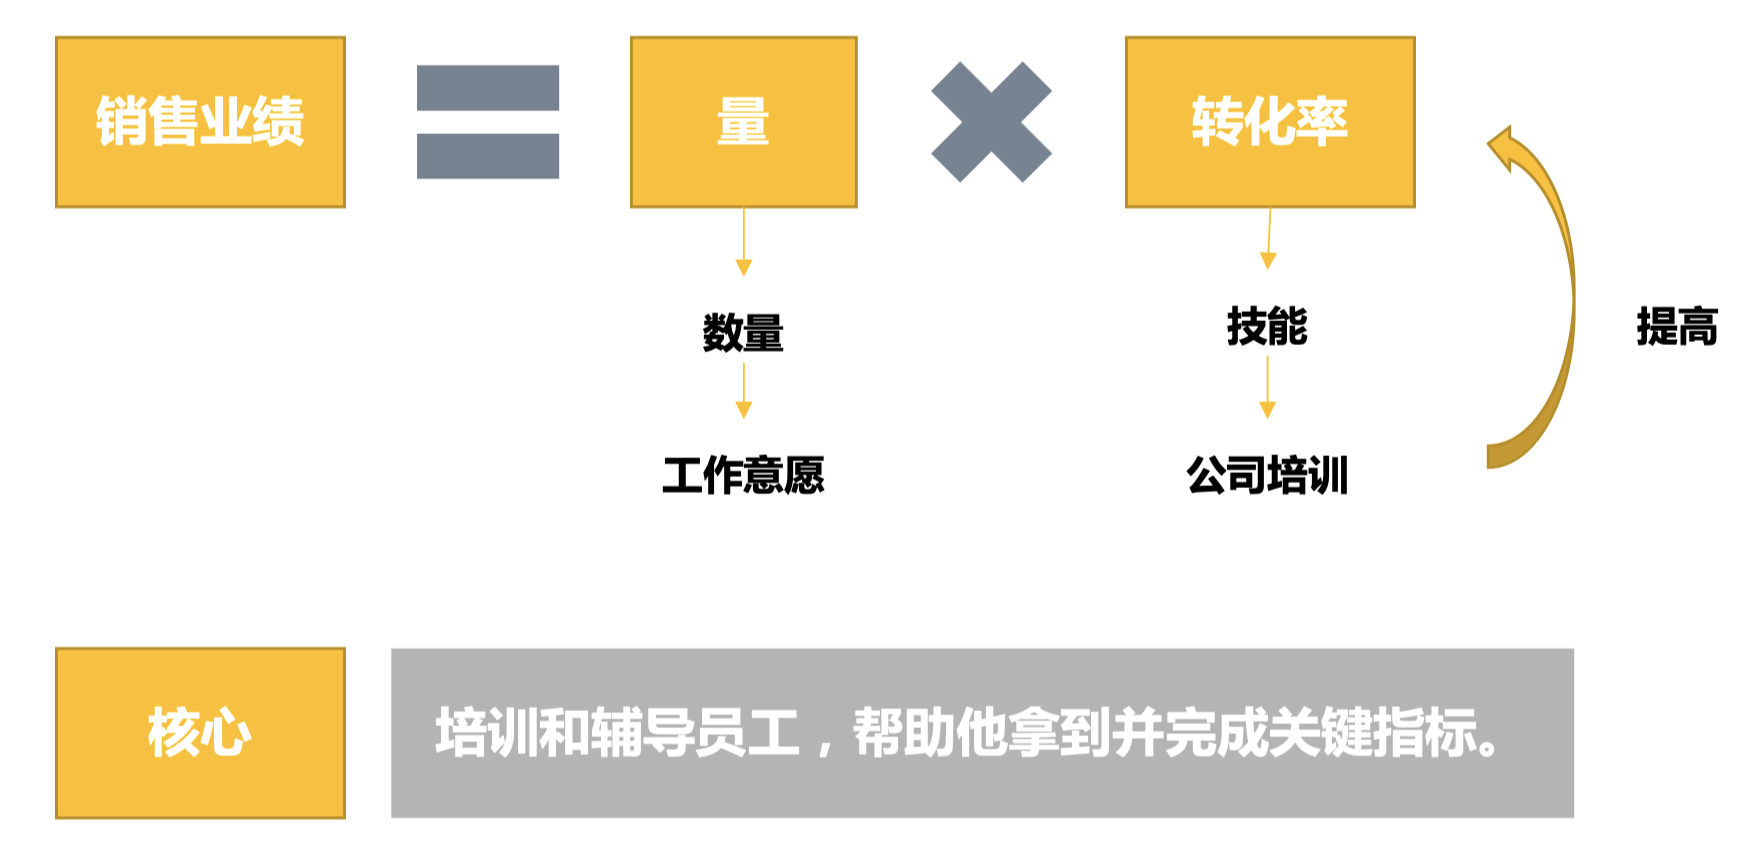
\includegraphics[width=1\textwidth]{fig/Ali_Performance_10.png}
\end{figure}

\section{阿里巴巴六脉神剑考核解读(中)}
\subsection{价值观解读与评估准则(六脉神剑全景)}
\begin{figure}[H]
    \centering
    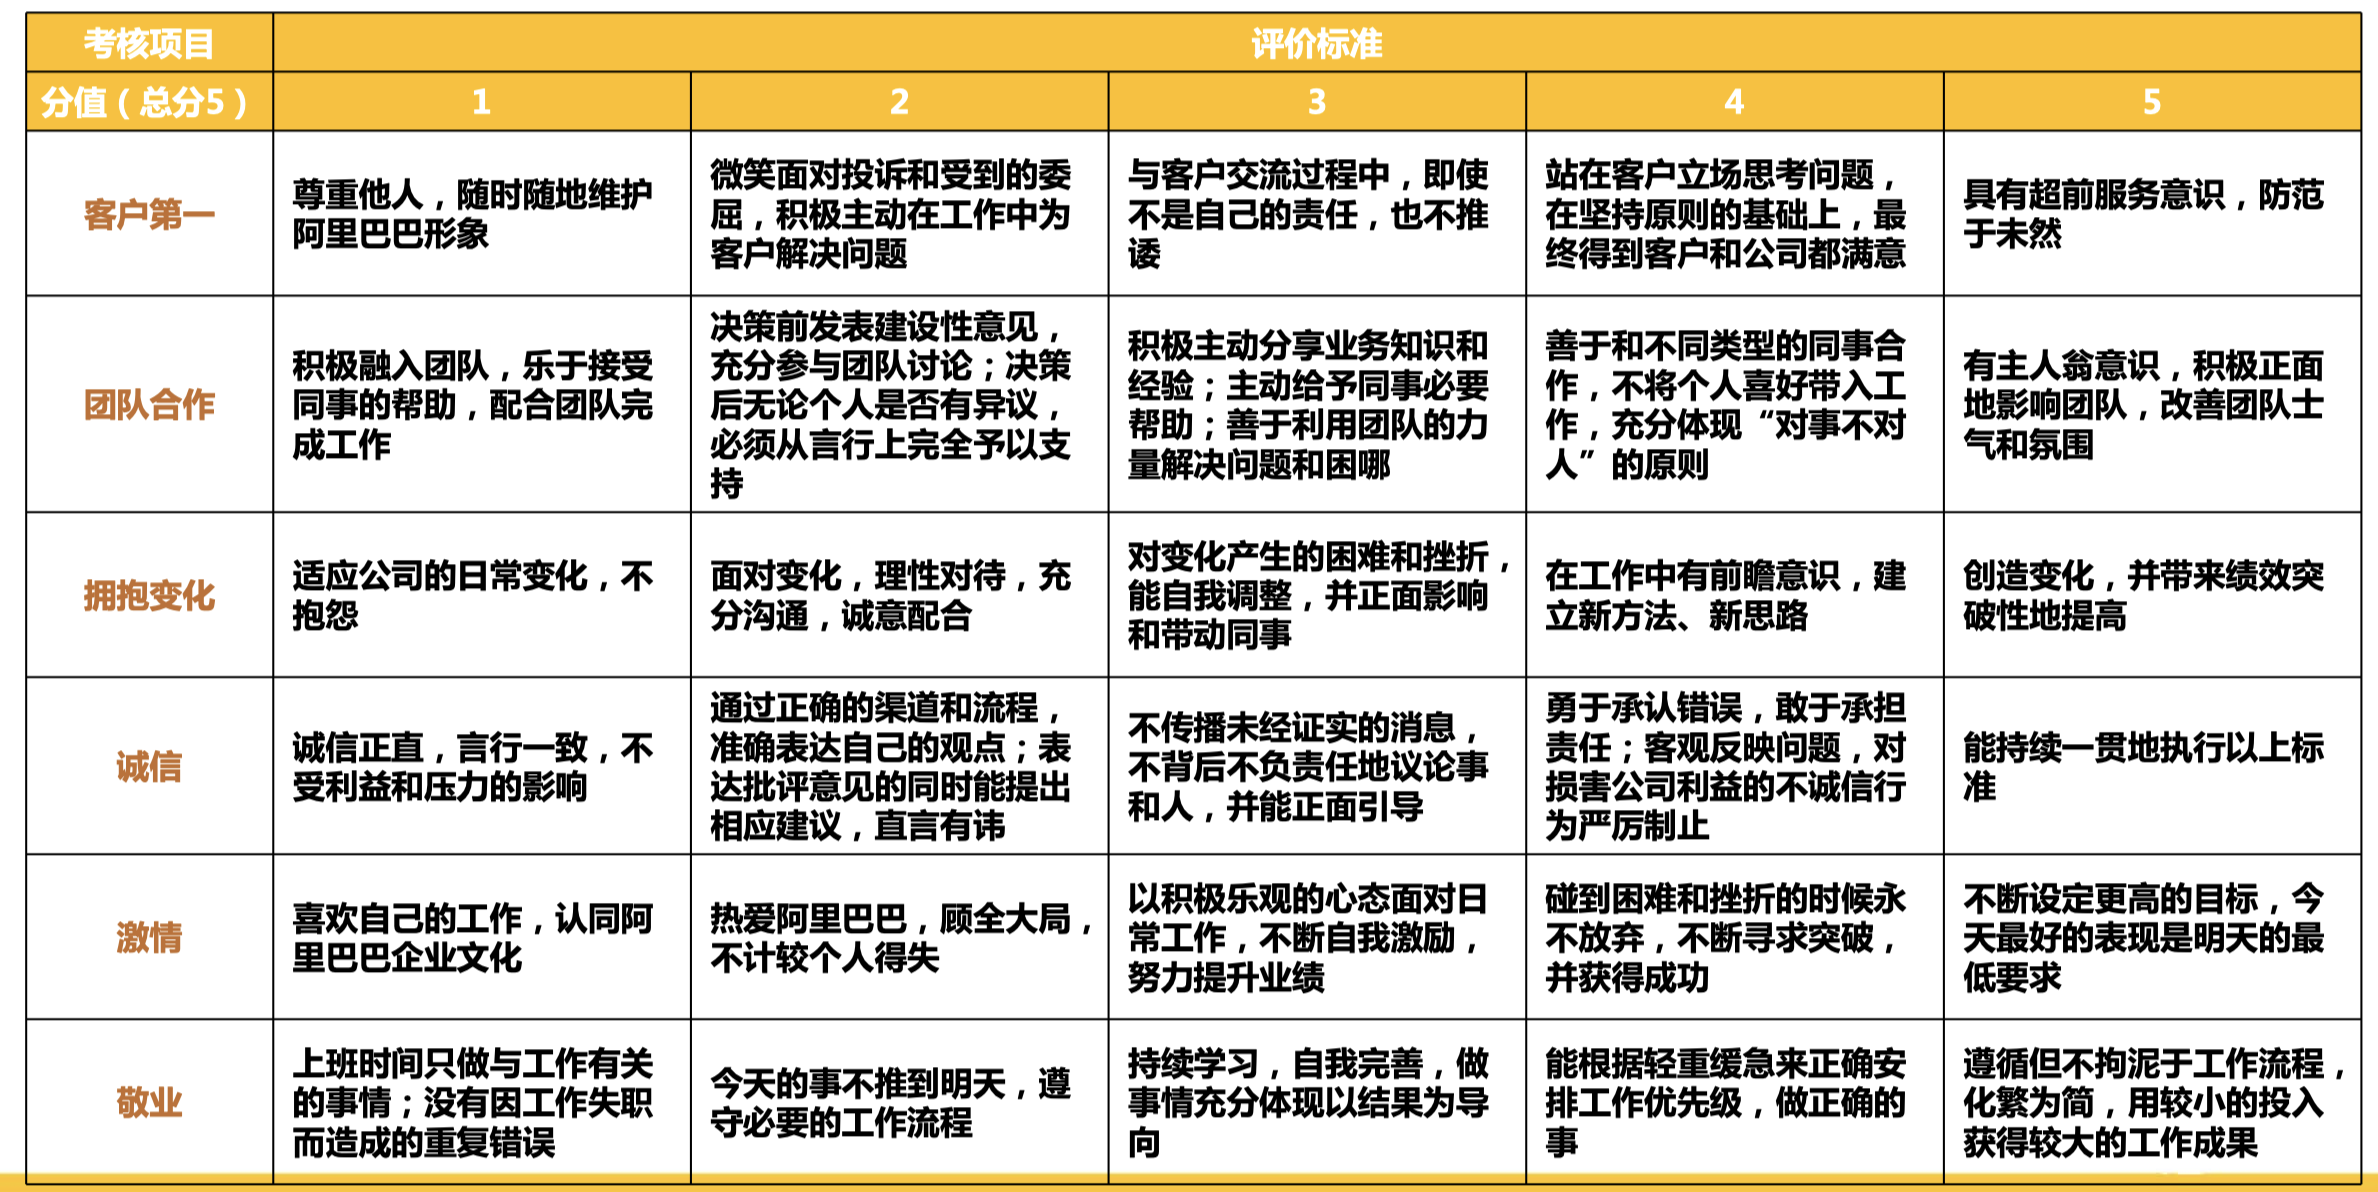
\includegraphics[width=1\textwidth]{fig/Ali_Performance_11.png}
\end{figure}

\subsection{客户第一}
阿里巴巴对6条价值观的打分,价值观落地,第1是有设计的理念,第2有考核的标准,第3有工作流程,第4就是价值观必须有诠释,怎么去考核员工,必须 要变成什么行为,这个行为是所有人一看就知道该怎么去做,否则根本就没有办法量化。所以如果我今天来打个价值观的打分,第1,价值观打分应该有什么 原则,第2,几分算不优秀,大家也知道,第3,价值观打分的一个组织原则是老板的老板和hr都要参与,我们一桌人在一起打分了,第4,怎么打分,逐条 打分,从1分一直打到5分。这个价值观是马总、关明生和彭蕾写了好几年写出来的,每一条都是斟酌的。凡是有逗号的地方都可以得0.5。精准到这个地方。

每一层都是递进的,第1层就是你客户第一的原则,是你要尊重所有的人,然后你要维护公司的品牌和形象,这个时候员工就知道怎么干了。 我们曾经有个 Top Sales是怎么被开掉的,就是在楼下跟保安无理取闹吵架,根本不尊重一个保安,吵得一塌糊涂,后来公司知道事后就把那个人给开了,因为你不尊重保 安。所以你只要尊重一个人,就是底层的视人为人,其实是没有层级概念的,遇到一个保洁阿姨也好,一个保安也好,一个客户看门人也好,你都应该尊敬 的,我们认为这是一个人最底层的素养。

第2分,我们经常会受到一些客户的投诉和委屈,要求你首先是微笑,因为客户来投诉你的时候,很多人会着急,就会跟客户对着干,但你要得到2分的话, 你得先微笑,然后积极主动帮他去解决问题,可以得两分。

这2分有了以后,我们怎么得到3分呢,在客户,比如今天客户来投诉个问题,明明是别人的问题投诉到你这里了,你说对不起,这不是我的问题,这是他的 问题,你找他去,如果这样,你这1分就没有了。因为客户的问题是所有阿里巴巴人的问题,这个时候你应该说好,我收到你的问题了,我们内部回去沟通一 下,看看怎么样立刻帮你解决,不会去推诿,说这不是我的责任,这条太重要了,做到这个事儿就是3分。

那么4分就很难了,站在客户的角度思考问题,基本上你能做得到个0.5分,但是在坚持原则的基础上,最重要达到客户和公司都满意。比如,这个事情处理 了,客户是满意了,公司受损害了,这0.5分没有了。但如果说公司满意了,客户不满意,0.5分也没有。

5分基本上不用看,是一个指导性意见,永远没有人打过这个分数。所以你发现客户第一不知道怎么做的时候,有这些行为的诠释,你就比较了解该怎么做了。

\subsection{团队合作}
第二条价值观团队合作,很多同学说我应该得5分,你看我影响了团队积极正向的氛围。但有可能这个人是一个空降兵来了以后,他根本就看不起,说你们这 帮老人太土了,我根本不想跟你融合。 这个人应该得几分?0分。所以团队合作最难的是彼此看不上,不融合,然后唧唧歪歪一堆声音,互相根本就不认同, 一大堆声音,执行力没有办法强。

所以我们会非常严格的规定,首先你到任何一个团队,基础分是你都得主动走向同事去跟他交流,应该是主动融合,这才得1分。

2分,在一般的公司都做不到,我们在决策之前大家充分讨论,你可以say no,他也可以say no,所有人都可以say no。但如果我们今天办公室达成了共识, 你出去以后必须在言行上百分百支持,再也不能出现当时这个决策我是不同意的,你们拍板定的,都是强迫我的。 如果你听到这个声音,肯定他这分就没有 了。这对团队特别重要,我们特别鼓励民主,就是大家在决策之前应该充分的讨论。但是很多时候团队里最麻烦的事情,达成共识再落地时候,很多人就不 认了,他翻脸不认,我就不同意,我当时也没听清楚,你们是用权力来压迫我的。他会很多的不同的声音,但不同的声音会导致这个事情执行落地就落不下 去。所以就是2分。

第3,积极主动分享业务,就是我们刚才说的教学相长,我会什么东西,我主动给你们讲讲,我有会什么东西会主动给予同事帮助。

4分的话,各种类型的人我都能合作,我不能够仅仅跟我喜欢的人去合作,这是鼓励对事不对人,所以我们就鼓励任何事情你们都讨论这个事情本身对和错, 不要跟人去关联,说这个人不行,不要去说,你要讲这个事儿对还是不对,这样就会变得特别简单,人跟人的关系就是处理事的关系。 这个就是团队合作。

\subsection{拥抱变化}
第三条,最有特色的叫拥抱变化,因为我们天天变,为什么员工都能够接受?换另外的公司绝对不可能,所有的员工都造反。但我们有价值观的正向引导和说明以后,你发 现所有的员工都能够接受变化。一个制度背后就影响了行为,行为时间长了就变成了一种习惯,最后拿到了结果就变成了思维的改变。

举个例子,以前我们在管业务的时候,阿里有两个现象,1个双职工特别多,第2所有的人都特别晚婚,因为我们以前在管业务的时候,只要是区域经理以上,有调动制, 在任何一个区域,都不会让你干超过两年。你这个区域干得好,再试试另一个区域,如果都能干得好,你就是优秀的,如果只能在宁波干得好,在广东干不好,说明你不行, 就不能晋升你。所以会告诉你说,必须有区域调动你才能够晋升。但背后还有一层意思是为了组织的安全,不可能让你成为一方诸侯。我记得每年到年底的时候,你一定会 走进老板办公室,说老板,我今年在厦门,明年我去哪,老板说明年你去东莞。好知道了,走了一句话都没有。

我创业的时候,第一站并没有选杭州,因为杭州都是熟人。我就觉得要做互联网的话,肯定要在北京,所以我就一个人拖个箱子来北京开公司了。 因为我以前就是这样, 开区是我一个人去。第1件事情把hr招到跟我一起干活。第2件事租办公室,第3件事去市场调查,摸底客户有什么需求,北京跟上海有什么不同的打法,摸完了就开始招人。 我们每个城市总为什么出来都能变成一个独立的CEO,就是因为每开一个城市的时候,基本上都是从无到有。这些人又不是铁人,为什么能做到,背后是价值观潜移默化的。

第1条就是不抱怨,我们第1次会不抱怨,不可能,我是浙江人,调广东去,我肯定是不愿意的。但是我想抱怨的时候,0分了,不行我就先闭嘴。因为我没有时间去抱怨, 我也没有机会抱怨,所以我得干马上抓紧去了解这边的情况,看看我怎样把它做好。所以你就开始把思想都集中在积极的地方,去想城市的策略,城市的目标,团队该怎么 招聘,该怎么管理,就往后做。 时间长了以后,制度这个行为我们就取得了很好的结果,因为我们每开一个城市都特别成功。

然后但这一条,我觉得全国调动这条阿里是比不上华为,华为更牛,华为是全球派遣。所以每个公司每年是不是业务都在变化,是不是人员都在变化,什么时候你公司会发展不前?当你发现没有办法对人事进行调动的时候,根本就没戏,你调不动你的人的时候,你已经没有办法玩这盘棋了,管理就是管人,人的这盘棋叫做铁打的营盘,流水 的兵。人你都调不动的时候,你还能干嘛?你不就是空有老板的名吗?根本干不了别的事。所以这是非常重要的。

\section{阿里巴巴六脉神剑考核解读(下)}
\subsection{诚信}
什么叫诚信呢?在阿里对诚信的解释1分是言行一致。你们跟阿里的人接触的时候,你们经常会怀疑这些人的智商和情商怎么能干活呢?因为他们基本上都是一根肠子通到底,基本就是想什么说什么,就做什么,脑袋里没有那么多复杂的东西。为什么?这是我们的价值观,我们就不喜欢复杂的人事关系,就喜欢大家简单的在一起创造梦想。

2分特别重要,通过正确的渠道和流程反映自己的观点。对任何一件事情有意见,我可不可以反馈?绝对可以,但是向谁反馈?向你的老板和hr反溃,但是不要向自己的下属去反馈,就变成抱怨了,人家搞不清楚,你想说什么,他又不得不奉承你,所以要有个正确的渠道。跟下属聊,聊不出什么东西来。后面,表达批评和抱怨的时候,一定要提建设性意见。在阿里高管有个非常好的习惯,任何人来跟我抱怨一件事情的时候,第一反应是,非常好,谢谢你,你的建议是什么?当发现一个人是没有建议的时候,这个人的抱怨不要听,他只是来跟你倒垃圾的。做管理的级别越高,受的委屈越多,压力越大,有没有机会每天去做别人的垃圾桶?但是如果这个人看到了问题,已经想到了解决办法来提建议的时候,这个人是非常优秀的,要鼓励他提建议。这件事情非常重要,这件事情会杜绝组织内特别不好的习惯,叫打小报告。是不是有人经常给老板耳边风,老板的耳根子软,听进去了,下次那个人过来,他就拿有色眼镜看他,脑袋里就在想你是不是这样一个人,是不是就是这样子。所以我们告诉你,不要来打小报告,要来反映问题。这个2分是不是太重要了。从此公司没人打小报告,因为打了也没有用。

3分也很重要。组织里面是不是有种特别不好的氛围,叫做背后议论人,种氛围会导致很多人特别难受。举个例子,你在公司里面,除了老板以外,你们有没有人被别人议 论过?你被别人议论的时候,你是什么心情?挺委屈的,挺气愤的,这种背后不负责任的议论,会导致很多正向的员工会离开,因为他承受不了心理的负担。所以我们特别 强调不传播未经证实的消息。只要不是公司官方宣布的,都叫未经证实。某某跟谁谈恋爱了,某某有盗窃的行为,某某有行贿的可能性,那个人能上位,因为他跟老板关系 好,当都是这种氛围的时候,大家心里都不会平衡。就没有那种蓝蓝的天,没有那种安全的感觉。所以组织的氛围要用硬的制度去保障,因为只有这样大家才会感觉倒是很 安全很舒服的。好的组织氛围背后都是有极强的组织制度在保障的。

后面这4分5分都不重要,反正一般都得不到,我一般都看前面3分到4分之间,因为我们想拿3.75分。

\subsection{激情}
激情,这也是我们特别喜欢的一条价值观,为什么你看到每个阿里的人出来基本上都很有激情,不管30岁还是50岁,为什么每个员工都会有那么有激情?

这条是我最引以自豪,因为这单条我得到过5分。迄今为止我一辈子觉得最骄傲的事情。你们知道员工为了得这个分数多么的不容易吗?拼上老命就是这种感觉,什么叫激情?首先应该热爱,比如我加入你们公司,我如果不喜欢,你觉得会有任何结果吗?没有。比如我是干销售的,但是我都觉得销售这份工作特别丢人,我根本说不出去,你觉得可能会有结果吗?所以任何事情的第1分是喜欢。

但我们的第2分要求很高了,不计较个人得失。比如我跟A因为跟客户吵架了,但最后上级判了客户给刘丽了,我觉得特别委屈,但我会不会找A算账,你分 一半给我,我有功劳的,这样的话就是开除。因为你私底下交易。

第3个积极乐观的心态,不断地自我激励。每天自我激励才3分。多少公司是老板激励员工,你快跑,快跑。在我们叫自我激励才得3分,4分就是永不放弃。 我们公司有一条价值观,是很多优秀人身上特别让我感动的,就是我们无论在开区域也好,做新业务的时候真的特别难。但我们有一条价值观是所有人认同 的叫做never never never give up,三个never,永不放弃。

第5条,今天最好的表现是明天最低的要求,今年你做一个亿,明年就是三个亿,永远是这样子,基本上我们每年的指标是不会低于百分百的增长的。 因为有这条价值观,你们看到每一季阿里的财报都在涨,挺可怕的。这么大的一个盘子还在涨,因为不长不行,我们价值观里有一条。所以这就是让每个员工都会觉得我永远在前进。

\subsection{敬业}
敬业。查一下阿里巴巴,包括华为和腾讯,员工制度里面都没有一条说你必须加班。作为老板,你们希不希望员工加班?不希望?你肯定不是老板,你太不了解老板了,所有天下的老板都希望,我付8个小时的工资,恨不得给我干18个小时,所有的员工都恨不得我拿8个小时的报酬,我干两个小时,这就是人性。

只要这个公司在快速成长,不可能不加班。我曾经做过测算,在互联网企业只要8点这家公司熄灯了,没有员工了,这家公司倒闭时间在8个月以内。那个时候互联网是个相对竞争比较厉害的行业,所以不可能让员工很舒服。 现在我们也比较倒霉,我们在北京的办公室对面就是阿里,当我们的员工每天出办公室 11点,发现对方灯火通明,每一层楼都开着,他们就很沮丧,说老板那边还在搞。这就是这条价值观,敬业的核心。

敬业第1分是,上班时间只做与工作有关的事情,没有因工作失职而造成的冲突。所以发现一个员工上班,如果说是看游戏,你可以让他走人。因为他上班做跟本职工作没有关系的事情,这是最不敬业的表现。

2分,今天的事不推到明天,遵循必要的工作流程。今天的时候不推到明天,你觉得我们的事干不干得完?我们以前老板会跟员工讲,你事保质保量干完了, 咱们6点下班。但如果说没有保质保量的干完,可能12点也走不了。但一个快速成长的企业事情多不多?做的完吗?这个东西框在这里,员工就是个永动机, 他干不完。如果说员工都五六点钟下班了,说明要么公司不行了,要么就是任务给他太少了,这个岗位可以裁掉了。

3分,持续学习、自我完善,做事情充分体现以结果为导向。所以没有结果的东西超不过3分,我们是要以结果为导向的。4分,根据轻重缓急来正确安排工作 的优先级,做正确的事。很多人会觉得看到第4条时候觉得特容易,优先级我都能排,但一看到2分就晕了。5分是遵循,但不拘泥于那工作流程,化繁为简, 用较小的投入,获取较大的工作成果。其实就是创新,创新是最难的。 但其实创新在阿里里面很多,为什么这一条从来没有人得到过5分,是因为前面两条 三条太难了,得不到,所以通关拿不到5分。

\subsection{阿里价值观诠释的目的}
1.任何一条价值观都应该有清清楚楚、明明白白的行为准则,让每个员工一看就知道该怎么做, 做什么是对的,什么是错的。

2.你要告诉员工每一条的正确的理解是什么,就像我是hr,我得给你们解读,叫传播价值观。 所以价值观是要传播的,我得不停的告诉你们什么东西是对的,什么东西是错的。

3. 阿里是打分制,不打分的公司更可怕,完全人治。老板说你行就行,说你不行就滚蛋,可怕。不要以为打分是残酷,不打分才是残酷的。我经常听到非常残酷,一个干了10年的工程师,老板脑袋一拍就走了,没有任何保障你。我们这套流程,就算马总看你不顺眼,也干不掉你。 一个制度健全的公司才是对员工最好的保障。

4.真正好的氛围是通过最严格的制度来保障的。 就像新加坡吐口痰罚死你,你会吐吗?不会。

\subsection{高管的胜任力九阳真经}
\subsubsection{胸怀}
• 领导者是寂寞的

• 胸怀是冤枉撑大的

• 心态开放,能倾听,善于换位思考
\begin{itemize}
\setlength{\itemsep}{0pt}
\setlength{\parsep}{0pt}
\setlength{\parskip}{0pt}
    \item[-] 领导人越往上走,就会越寂寞,这是一个必经的过程, 很多领导者会有很多抱怨,但是请提醒自己调整心态, 这是一个正常的情况
    \item[-] 做领导人一定要做决定,而很多决定是要力排众议的。 因为你处在这个位置,你看的东西要比别人多,反过 来理解你的人就会更少。在寂寞中找到不寂寞的东西。 要能耐得住寂寞,学会自得其乐,宁静以致远
    \item[-] 胸怀是冤枉撑大的,作为领导人,一定会有被冤枉的 时候,这也是正常情况,当被冤枉的时候,有胸怀的 人才能坚持
    \item[-] 胸怀首先是开放,只有领导人的沟通是开放坦诚的, 才能让下面的人也开放坦诚地沟通
    \item[-] 其次是包容,包容各种各样的人,思想和文化。要做 到包容,自己不要有太多先入为主的判断,要善于倾 听和换位思考
    \item[-] 上善若水,领导人最高的境界是如同水一样:水能高能下,流动中无形,但是旁边的东西是什么形状,就 是什么形状,至柔至刚
\end{itemize}

\subsubsection{眼光}
• 会看,看到别人没有看到的机会,防止灾难

• 会Sell,让大家都参与进来

• 有结果
\begin{itemize}
\setlength{\itemsep}{0pt}
\setlength{\parsep}{0pt}
\setlength{\parskip}{0pt}
    \item[-] 会看,机会和灾难都要看到。知未明,观未见:知道 别人还没有明白的,看到别人还没看到的
    \item[-] 战略是3分看出来的,7分做出来的。大方向对了,不断试错。好的战略是“苦熬”出来的。不管能否看清 未来的方向,至少自己要经常去思考,经常抬头看路, 而不是一直埋头赶路。会Sell,自己看到了,还要会 让大家对机会兴奋起来,对灾难重视起来
    \item[-] 眼光需要全球化。21世纪的成功领导人要素:开放、 分享、全球化、责任感
    \item[-] 有眼光,还要有结果。通过别人拿结果,通过结果不 断修正自己对方向的判断。要拿到结果,需要在组织, 文化和制度上相应支持
\end{itemize}

\subsubsection{超越伯乐}
• 找对人:知人善用,用人所处

• 养好人:在用的过程中养人,在养的过程中用人

• 养成人:造接班人,鼓励青出于蓝而胜于蓝
\begin{itemize}
\setlength{\itemsep}{0pt}
\setlength{\parsep}{0pt}
\setlength{\parskip}{0pt}
    \item[-] 善用人者,为之下。欣赏自己的同事,带人谦和,善 于从他们身上学习。不争之德者,为用人至上。不争之德,不以权力压人,不轻易发怒
    \item[-] 善于发现同事身上的优点,并用其所长。有意识地把 人放到给他更大责任和压力的地方,会让他成长得更 快。通过别人拿结果,通过结果培养人
    \item[-] 阿里巴巴的领导人要有老师的心态。凡事做领导的人, 应该把培养接班人作为首要任务,要有胸怀去找能够 超越自己的人
\end{itemize}

\subsection{价值观解读与评估准则(九阳真经全景)}
接下来我们来看一条高管,胸怀、眼光和超越伯乐。第1条胸怀。管理者是寂寞的,越高级别的领导你越寂寞,因为别人没有办法理解你,因为别人看不到你 的高度,这叫高处不胜寒。所以管理者是寂寞,是常态。只有老板能看到所有的东西,但你下面的人他只能看到一个尾巴,一条腿,所以他不可能完全理解 你。第2,胸怀是冤枉撑大的。第3个胸怀是说心态开放,能倾听,善于换位思考。就是说一个老板一定要能听不同的声音,因为有效的学习就是听到不同的 声音,听到相同的声音是无效的。领导人越往上走越寂寞,这是一个必经的过程。比如说你今天带技术团队,你是技术团队的老大,那么技术团队的业态, 就喜欢崇拜技术大咖,他不喜欢被拘束,你就不能像管销售团队一样去管这个技术团队,一定不认的。那你就以支持者的角色,尽量去做到学术的权威。但 如果说去带一个以结果为导向的部门,就是要变得很狼性,很血性,这就是你不同的业务业态要去变的东西。这个是九阳真经里面对胸怀的诠释。

每个人都受过很多的委屈,我讲讲自己的委屈,我在阿里经历过38个老板,原来我刚刚接触这么多老板的时候,心态是比较苛刻的。我觉得这么多老板里头 也就两个老板,真正在业务上帮到过我,在管理上帮到过我。 因为我自己觉得做业务是比较有天赋,其实不太需要别人帮助的。后来成熟的时候发现,其实 每个老板对我都是有帮助的,比如说像有个老板我记得很清楚,他虽然业务上没给我什么指导,但是他在平衡生活,处理人际关系特别好,我就学到了。我还有个老板特别会向上处理关系。我原来觉得这个人怎么天天拍马屁,我特讨厌他。后来我发现你领导做的越来越大的时候,能够管理你的老板是最重要的一件事。因为你作为一个部门总裁或者说公司总裁,如果你不能获得更高级别老板的支持的时候,你拿到的资源是很有限的,你就没有办法支持到你整个部门 的发展。 所以向上管理很重要,所以为什么去选拔一个高管,最好去挑那种在一个公司里面从底层一层一层一层往上升的人,这个人一直往上升的背后是他 一定是克服了无数的困难,无论是心态上、工作上,你知道一个人最难能可贵的是一个非常强壮的心态和他解决问题的能力,这才是高管的格局。一个能在 这么严酷的环境下能够生存下来的人,他的心态一定很强壮。他一定解决问题能力强,否则他活不下来。所以这样的人才具备一个高管的素质,1年就跳槽的 人说明这个人一旦进入深水区,就被别人发现这个人不行,他干不下去了,所以他得跳槽。大家看到这些本质的东西,一个高管是不是胸怀很重要?

\subsection{价值观落地总结}
第1,要把设计理念拎出来;

第2,提炼你的价值观,总得有价值观,没有价值观咋考核;

第3,要设计出自己部门或者自己公司的一套考核的机制。也许可能不是跟业绩挂钩,也许可能不是跟价 值观挂钩,但总得有个落地的方式,你知道你只有对你的管理干部越严格,他们会表现越好;

第4,当你价值观真的要变成每个员工的共识的时候,你需要一条一条把它诠释出来,一定要诠释成行为, 大家一看这个东西,他就知道该怎么去干。

\section{不同阶段,如何打造不同的组织能力}
\subsection{CEO是首席教育官}
第7个工作方法论叫做企业持续发酵的密码,有个核心是以使命愿景为核心,然后一定要 有个完善的治理结构,然后应该有个底层的文化体系,还应该有源源不断的人才培养梯队。

怎么样才能让你的公司源源不断地有人才?每个老板都喊,我没有人才,怎样让你的企业 有源源不断的人才梯队?只有一个答案,老板变成首席教育官。

上个礼拜马总退休的时候,他说了一句话,我特别认同。CEO,还有一个英文名字,E是 education,教育,首席教育官,我特别认同。所以老板变成首席教育官,每天孜孜不倦 在带你的下属,然后通过传帮带,一代一代往下传的时候,公司才有可能会有源源不断的 人才梯队,否则都是没有的。你靠谁去带?只有你把高管带好了,高管把中层带好,中层 把管理层带好,管理层把员工带好,才会有源源不断的人才梯队。

所以在培养人才梯队里面最重要的是你的张良和萧何。张良和萧何帮助刘邦打下了天下。刘伯温帮朱元璋打了天下。那谁是你的逍遥子?逍遥子帮马总 接了班,谁是你的关明生?帮马总打了天下。

\subsection{阿里巴巴的例子}
举个例子,逍遥子第1天进来就能够把马总的班给接过去吗?不是的,逍遥子是07年到公司的,他是做财务的,一件一件,一仗一仗的胜利打过来之后,公司 给了他所有的培养,他参加过所有的管理培训,每年的梯队培训,马总亲自带。这个人,是在公司被培养了10年,现在才接班的。

我想表达的一个是,谁是你的人才,这个人才你是需要培养的,就算你空降进来个高管,也要培养,因为你要让他的文化跟你契合,你要他非常了解你的公 司,然后他要内心从了解文化,到感知,到沉淀,到变成他自己的信仰,这个轮回是一定要的。马总选接班人,一定会选极度信仰它的文化的人,一定会选极度有能力的人,一定会选极度有领导力能服众的人,这些人就是千锤百炼。第2,他比很多老阿里人都更加热爱公司。你也奇了怪了,一个财务的老大,比 业务的老大还会算账,还会做业务,什么天猫战役,他从来没搞过,都搞起来。 所以他后来接了我们的班,所有人都认为接班人应该是他。逍遥子不是阿里 的老人,他是个空降兵。

所以人才梯队,1,你要想有源源不断人才梯队,你做老板的必须,要承担价值观的,教学相长,你要承担老师的角色,并且要在公司内部倡导,你做我老师, 我做你老师的这种学习的氛围。第2,人才梯队,就是一届一届班有人接,一层层,你不要忘记谁是你的逍遥子,谁是你的张良萧何,这些人都是需要培养的, 不是说拿进来马上就变成你的接班人。今年你给公司内部培训,超过100个小时的你很优秀。老板如果不花时间在培训上面,你们公司永远不会有人才梯队。

这句话特别贴切,用人唯才,量才而用,人所共知,说易却行难,这个道理谁都明白,每个人要用的都是人才,然后要根据每个人才放在合适的位置上去用, 所有人都明白这个道理为什么做起来这么难? 因为他要花你的时间和精力。所以老板你的时间花在哪个地方,哪里就会有产出。

\subsection{组织发展与个人发展}
\begin{figure}[H]
    \centering
    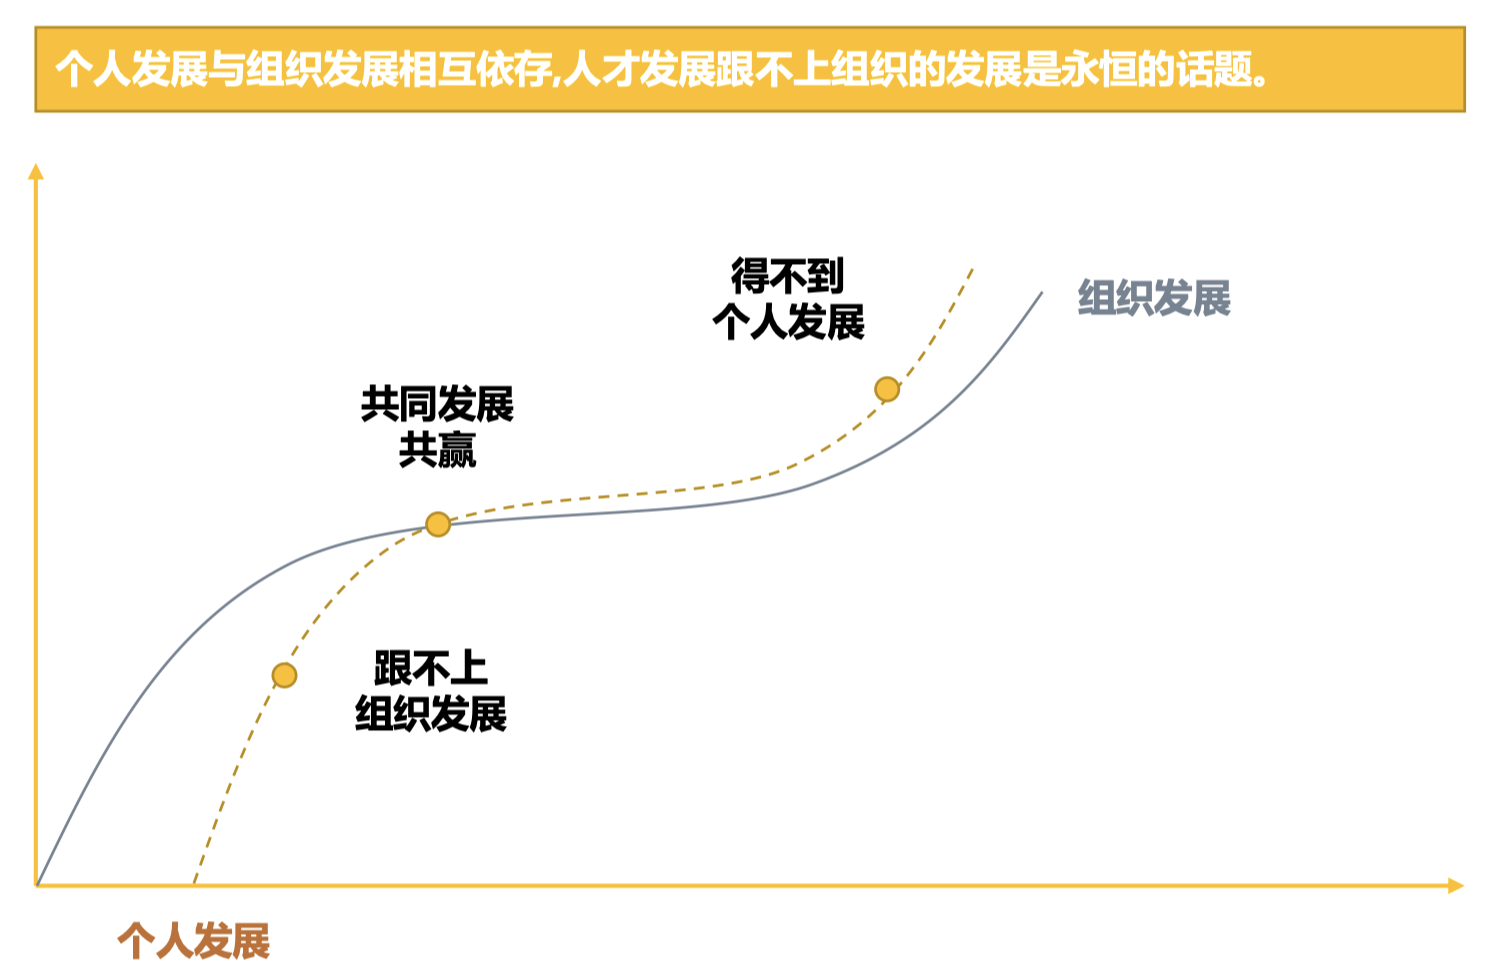
\includegraphics[width=1\textwidth]{fig/Ali_Performance_12.png}
\end{figure}

大家看一下这张图,你会发现人才发展和我们公司的需要永远是不匹配的。只有一个点上是交集的,绝大部分你会发现都是不匹配的。举个例子,人 才离开你公司,除了价值观的问题,只有两个原因,第1个原因,公司发展太快了,他跟不上,他掉队了。第2个原因,公司发展太慢,他看不上公司, 他就离开了。这是员工离职的本质,我们曾经分析过。 个人发展跟不上公司发展和中间有落差,是一个永恒的话题。

这张图表达了两个意思,第1,人才发展和组织发展相互依存。我们所有人的发展都是 要根据业务的需求在增长的,所以这两个是相辅相成的,你没有公司非常清晰的发展 目标,就没有清晰的人才发展目标。第2,人才发展跟不上公司发展是永恒的话题。只 有创业公司是这样吗?难道大公司不是这样吗?所有的公司都面临,永远是人跟不上 公司的发展,我今天公司要转型了,从硬件转到软件,我人跟不上,我今天要做飞天 的事业,像阿里一样想飞到火星上去,没有这样的人。百度想转型,没有更多的陆奇, 所以这是个永恒的话题。人才发展永远跟不上组织的发展。

\subsection{组织发展的四个话题}
组织发展我们讲4个话题,第1个话题,组织发展,公司要做下来,就好比是企业打天下,第2个企业不同的周 期,我们需要打造不同的组织能力,第3,组织发展需要有4个要素才能发展。 第4,组织发展,也需要有落地 的保障机制,才能够进行组织发展。

企业打天下,这个图大家记住,从天到地,每一个都要做,才能够把江山打下来。这就是关明生那本关乎天下 的书,里面通篇讲的东西,这是我最喜欢的。0~3000人的公司发展特别适合,你只有CEO带着高管把所有的 事情从头到尾都做一遍,才有可能把天下打下来。最核心的是,不同的业务的愿景使命决定了不同的战略,不 同的战略决定不同的组织架构,决定了不同的组织能力,所以一定是不同的愿景导致了不同的战略导致了的架 构,不同的架构下我们想要打造的组织能力,全部都是不同的。

\subsection{企业打天下}
\begin{figure}[H]
    \centering
    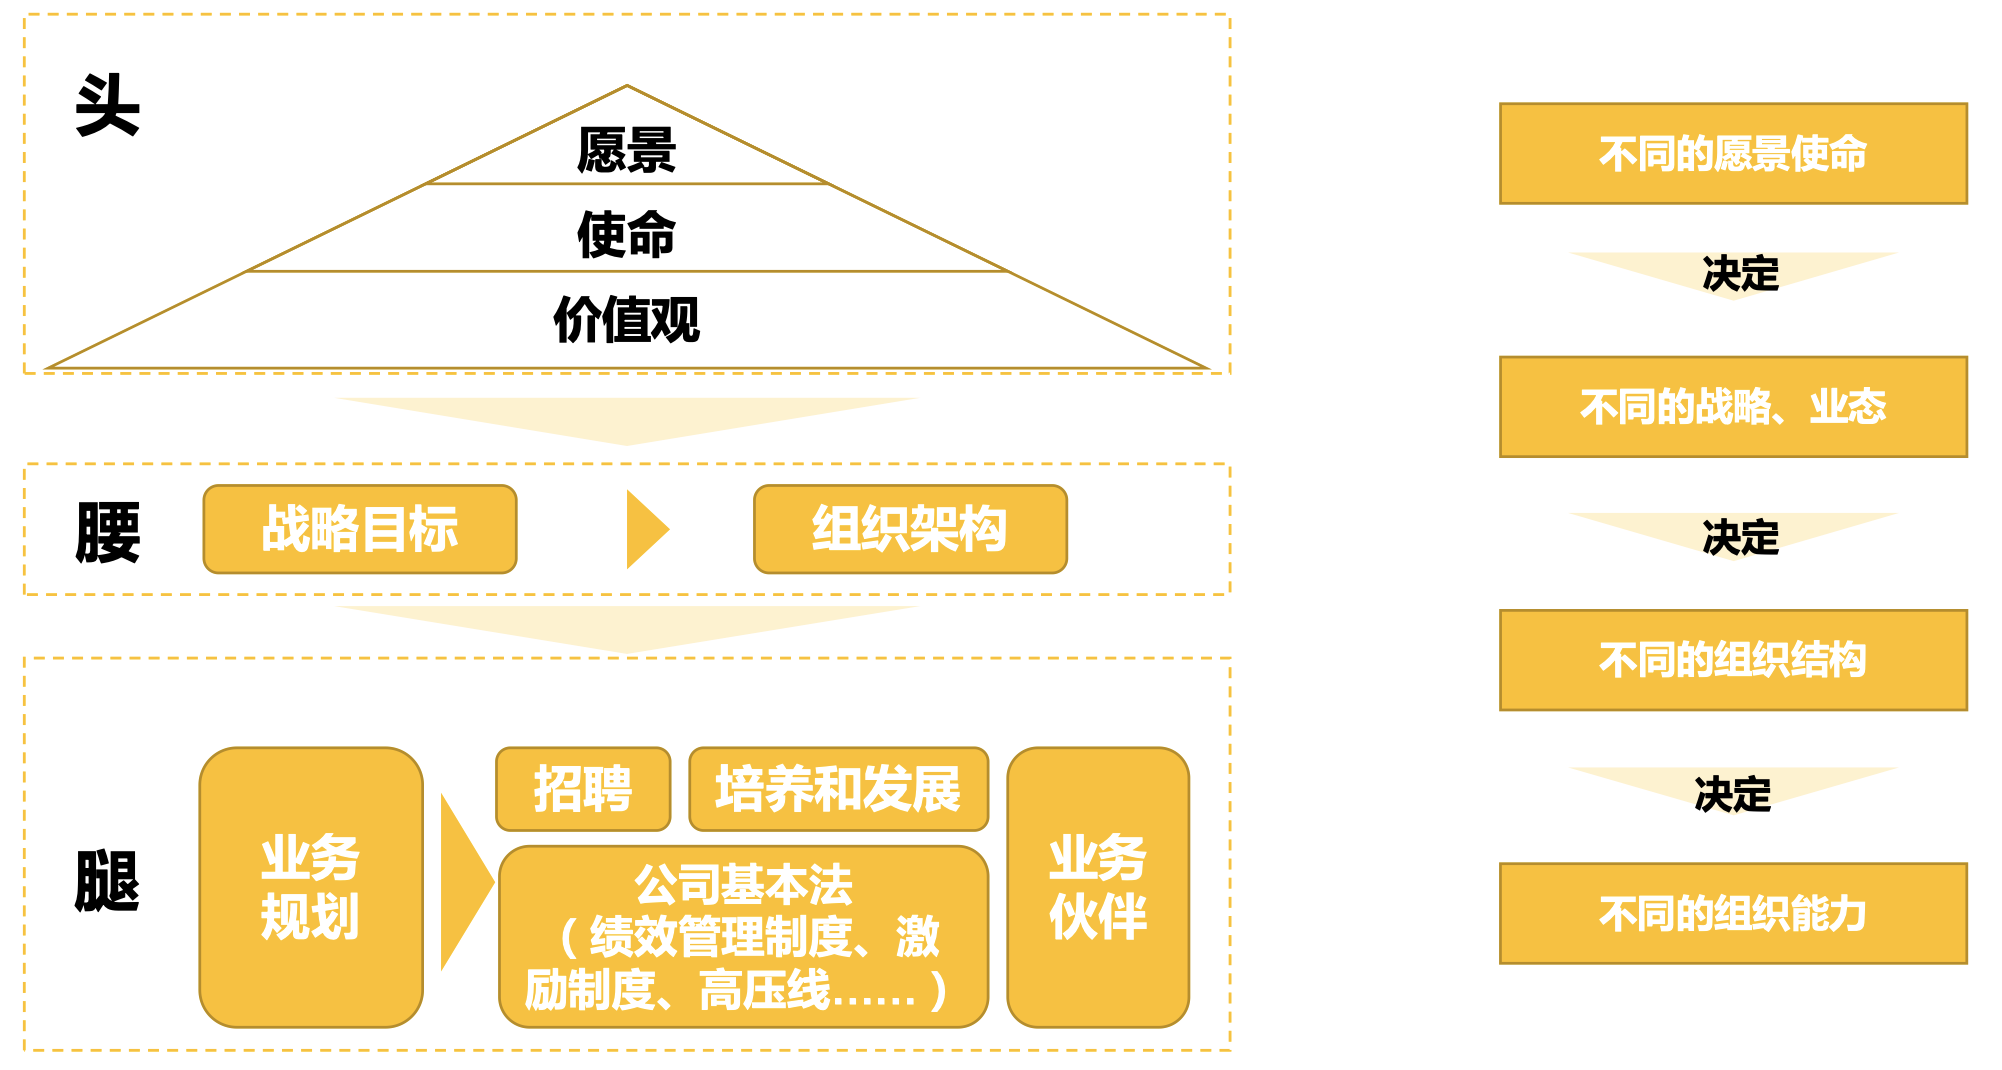
\includegraphics[width=1\textwidth]{fig/Ali_Performance_13.png}
\end{figure}

\subsection{企业不同生命周期需要打造不同的组织能力}
\subsubsection{初创期 0~1 —— 生存}
• 大浪淘沙,剩者为王

• 选拔比培养更重要
\begin{itemize}
\setlength{\itemsep}{0pt}
\setlength{\parsep}{0pt}
\setlength{\parskip}{0pt}
    \item[-] 公司在草创的时候,0~1,在0~1的时候,我们最需要的文化是生存,围绕着生存,我们要打造什么样的组织能力?组织能力的概念,是一群人的能力,我们是要打造一群 人的生存能力。如果要让你的团队有生存能力,需要培养他们什么样的能力,这些人才能生存?签单,做业务吧,你得赚钱,你肯定要培养大家赚钱的能力,你不培养大家 赚钱的能力,怎么生存,还有要结果导向对。所以这个时候你会发现,组织能力是要围绕着你的阶段来的。所以在从0到1的时候,我们要打造的组织能力,围绕着生存走 的,我怎么样快速的能够把单子签下来,我怎么样能快速的回款,我怎么样能做到客户第一,能够把钱给我收回来,客户能认同我这些东西,这些能力都是创业初期的能力。
    \item[-] 所以早期你会发现在创业公司最多的培训,如果你们公司有销售团队,天天培训销售怎么去签单,假如你们公司是以产品为驱动的,你就天天去打磨你的产品,尽快把产品 给迭代出来,这就是咱们0~1要培训的东西。但这个时候告诉大家,培训不是最重要的,最重要的是什么?大浪淘沙,剩者为王。因为一家公司最早期的时候,你剩下来的 火苗,应该是最优秀的人。最优秀的人有可能不是学历最高的或者最资深的,而是这个人最具有奋斗精神、最能吃苦、最能跟你同甘困苦的人。他最有理想的人,你要把这底层的人给他筛出来。这层人怎么筛?效率最高的,组织管理在0~1的时候就是大浪淘沙,剩者为王,阿里每一期七八十个人,就剩下那么3,4个,这3,4个人一定是好 的,第1,业绩能做出来,能给公司赚钱,有能力。第2,这种心态和压力之下,这个人压力是不是很高,他留着可不就是喜欢公司。
    \item[-] 所以早期的组织能力最需要的是快速循环,快速循环。这里很关键的是选拔比培养更重要。
\end{itemize}

\subsubsection{扩张期 —— 稳定}
• 大浪淘沙,剩者为王

• 选拔比培养更重要
\begin{itemize}
\setlength{\itemsep}{0pt}
\setlength{\parsep}{0pt}
\setlength{\parskip}{0pt}
    \item[-] 第2阶段,公司到了快速增长期。快速发展期最大的特征是乱,太乱了。最危险的时候就是扩张期。讲一个故事,有家公司融到5个亿,6个月之内关门,也是我亲身经历的。 我刚从阿里出来的时候,投后管理,当时的一家团购公司,融了5个亿。当时这家团购公司和美团、窝窝并列前三,一个月的销售额4个多亿,融到了5个亿,为什么这家公 司在6个月之内关门关掉。我第1天去见企业老板,老板跟我讲,我们打算用半年的时间赶超阿里,我说什么地方能赶超阿里,他说人数规模,我现在已经是6000个人了, 我平均一个月进1000个人,我再过6个月可不就12,000人了吗?阿里B to B团队不也就6000个人,我肯定就干掉阿里了。这是老板跟我讲的第1个观点,老板是个海归, 绝对的精英,哈佛毕业,一天睡三个小时,充满了华尔街的荷尔蒙。极度的聪明,极度有进取心,充满了野心,学习能力没有人比他更强。这是第1个问题。我当时给老板 的回复是,我害怕,我跟他说你一个月能进1000个人,你进的人一定都是乌合之众,我不相信今天哪个公司能够一个月招来1000个人全是优秀的。第2,招聘不是你想招 多少人招多少的,而是我内部有多少管理者能够去管这些人,否则永远出乱子。
    \item[-] 第2问题我再跟他共事的时候,发现他一个结构性,系统性风险是,它全国有100多个分公司,分南北两个大区,南总监、北总监。南北总监下面各管10个大区,一个大区 下面管10个区域,100多个城市,他们当地所有的hr,所有的财务都是汇报给当地的城市总的,有没有系统性风险?我说这绝对是系统性风险,他没有理解。
    \item[-] 第3,当时这个公司有个特别优秀的地方,文化做得非常好,因为他们天天学阿里,学毛选,每个礼拜五CEO亲自带队,大家学管理,这是我特别喜欢他们的地方,就是每 个礼拜五晚上,周会一开完,所有的高管聚集和过来,老板带头学,所有的管理学,拿着一本书就开始,你念一段我念一段,氛围特别好。我去他们公司的时候,第1次他 们200多个管理者坐在这里,我也是我给他们上了半天的管理课程,我能看到那种蓬勃的朝气扑面而来,这种血性的东西扑面而来,真的是一个非常有战斗力的团队。
    \item[-] 这家公司的文化非常好,人才有很多,年轻人90后的也很棒,人才梯队也有,死在哪里?公司三角形人才梯队和文化的上面是治理结构,很重要。第1个招来的人,后来被 我发现了招聘总监外面有自己的两个招聘公司。这个招聘总监,当年是跟着老板,但是这个人原来是做裁缝的。从这两个信息可以判断出来,第1这个人有没有专业度?第 2个,这个人用自己的招聘公司,往公司倒人,这个人有没有职业度?可以得出一个结论,他招来的人肯定是不行的。一个月1000个人呜泱泱进来,是什么样一种状况? 第2,我刚才说了一个非常重要的信息叫治理结构,每个分公司的hr和财务是跟老板汇报的。在后面就遇到了巨大的问题。这是8月份的状况。
    \item[-] 10月份的时候,南大区管了10个区,50个城市的总监,突然被竞争对手搞定了。然后竞争对手给他出了一个主意,你过来然后把你下面10个大区全给我弄过来,然后总监 就把这大区经理叫过来逐个击破。当时总监的风格,这个人没有管理套路,没有管理体系,完全是靠兄弟情义,兄弟咱喝两瓶白酒,咱就是兄弟,是用兄弟情谊去管理公司。 我喜欢理性的管理者,很多理性的管理者背后是很有爱的,是用管理体系在管。就算你不合格,即使是马总也不能随便辞退人。体系化的管理是避免系统性风险。整个南北 大区的风格是完全不一样,北大区的老板全是体系化管理的,现在是美团非常重要的一个人,南大区的老板全是靠兄弟情义管理的,所以你知道他选拔的大区一定是跟他有 非常亲密的关系的人,一切以人际关系为纽带,而不是以专业度为纽带。他用一个礼拜的时间把10个大区总全部搞定,开始叛变,叛变的时候一夜之间所有的管理层走光, 所有的钱全部卷跑,因为财务是汇报给当地区域经理的。我们后来发现当地的区域经理和hr老大都是亲戚,公司又没有任何监督。阿里严格强调,hr、财务线一定是集团 总部直管,三权分立,否则你就是土霸王,谁能管得了你。所有的财物全部都卷了,人也是他们的人,恶劣到偷偷的给所有的客户放消息,说这家公司要倒闭了,赶快来结 账,结果一个月之内,所有的商户到分公司打砸抢。一直到12月份的时候,老板真的撑不下去了,最后宣布公司破产关门。12月底的刚过完圣诞节的时候,清的盘子。
    \item[-] 我看到这家公司是8月中旬,8月底给他们做了培训,我想表达的,扩张期是最混乱的,所以我们需要的关键词是稳定,怎样能做到稳定?治理架构。为什么要做学习发展, 要统一思想,不能1000个人进来后全是乱七八糟跟你们思想不一致的人。老板请你们去搭建自己的体系,因为你不建体系永远混乱,永远过不了这个阶段。
    \item[-] 死的最多的永远是快速扩张的时候,因为0~1的时候,每天过的都是如履薄冰。但到快速成长的时候,账上有了一些钱,公司有了一些人马,自己像个老板的样子。很多老 板每天门口一堆人排着队请他签字,特别享受那一刻。以前鼎晖投资有个数据统计,99\%的民营企业死掉的时候,老板有两种选择,一种让公司活,另外一种让自己爽, 爽有很多层含义,什么权威性,我来做主,按照我的意思想法,以我为核心了。99\%的企业家选择了让自己爽,所以公司就死,所以大概率的死亡全是发生在快速扩张的 时候。所以在这个阶段一定要注重稳定,把公司规章制度物,各项体系搭出来。第2,把你们公司内部的培养计划定出来,人才培养计划,否则就很麻烦,死的太多了。
\end{itemize}

\subsubsection{成熟期 —— 变革}
• 自内而外长出来

• 三层能力变迁
\begin{itemize}
\setlength{\itemsep}{0pt}
\setlength{\parsep}{0pt}
\setlength{\parskip}{0pt}
    \item[-] 到了成熟期,我们需要什么样的组织能力?破局,我们需要变革,但变革非常重要的是由内而外长出来才是有力量的。一个公司他如果自己的内力不够,就 完全依托外面的力量敲敲打打说你要变革,你觉得这个事靠谱不靠谱的?所以为什么我说变革唯一的可能性是老板自己来提,否则没有可能,因为变革的力 量必须由内而外的生出来,才有可能会长得出来。成熟期最核心的是由内而外的变革驱动力,不是外部的,没有用。
\end{itemize}

\subsection{组织发展的四要素——阿里巴巴组织发展案例}
\begin{figure}[H]
    \centering
    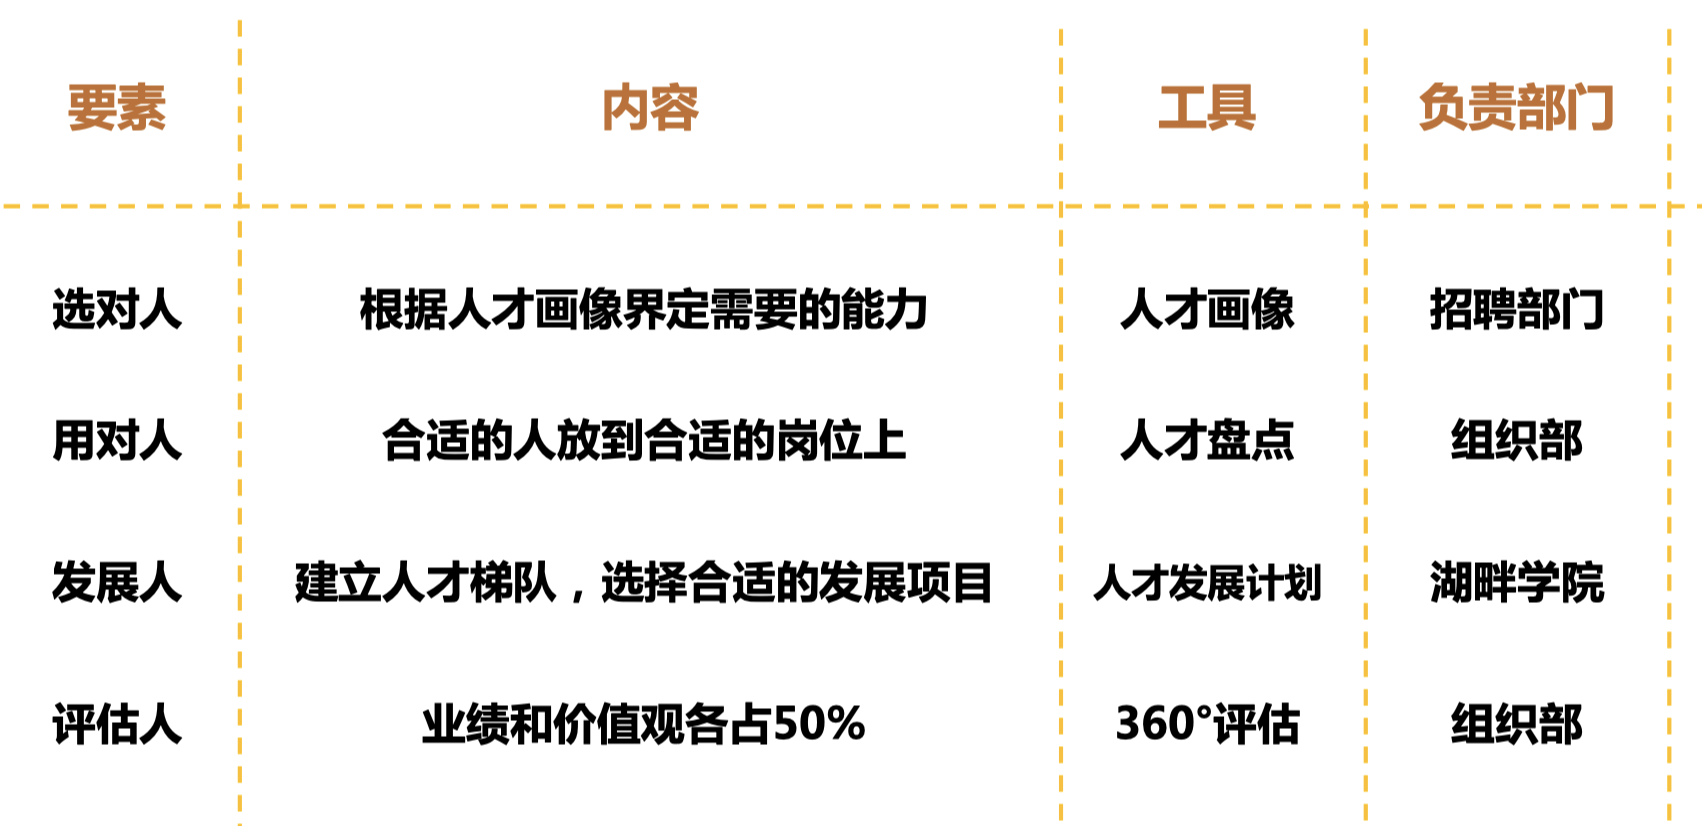
\includegraphics[width=1\textwidth]{fig/Ali_Performance_14.png}
\end{figure}

组织发展的4个要素。组织发展到底指的是什么?第1,叫选对人,选对人就是我们上次说的招聘,所以是要根据人才画像,根据他的胜任力去定能力,负责部门是招聘部门,但这个部分真正的主人是业务部老大,不要忘记了招聘是咱们自己的事儿。

第2个要素,选对人以后是用对人,用对人就是把合适的人放在合适的岗位上,有个工具叫人才盘点。 举个例子,在阿里人才考评部叫做叫组织部,在华为叫干部管理部,小米也成立了组织部,就这个部门专门来负责管理干部的考评。普通员工就各个部门自己考评。

第3,发展人,发展人就是建立人才梯队,老板亲自带队来建立人才梯队,选择合适的发展项目,有个工具叫做人才发展计划。类比一下,这就是阿里巴巴的湖畔学院干的,是内训的领导力部门干的。

第4,评估人叫绩效考评,对阿里来说高管是组织部考评,下面的人就是one over one plus hr。

所以在整个组织发展的4要素当中,核心就是选对人、用对人、发展人、评估人。

\subsubsection{用对人——人才盘点}
人才盘点最核心的就是这么几个事:
\begin{itemize}
\setlength{\itemsep}{0pt}
\setlength{\parsep}{0pt}
\setlength{\parskip}{0pt}
    \item 第1,根据不同的业务业态,设计出组织架构。
    \item 第2,根据组织架构去定 每一个岗位的职责。
    \item 第3,划出每个岗位职责的胜任力。之后第1件事,可以根据 胜任力,看看我们这个组织里面有没有这样的人,没有的人 应该去招聘。第2,看到我们现在的人跟胜任力的差距,去做 培训。第3,考核也一样,可以根据胜任力跟现在人员的对比, 决定去晋升谁,决定淘汰谁,去换掉谁,都一样。
\end{itemize}

\subsubsection{案例:不同角色的不同定位(岗位定义)}
\begin{figure}[H]
    \centering
    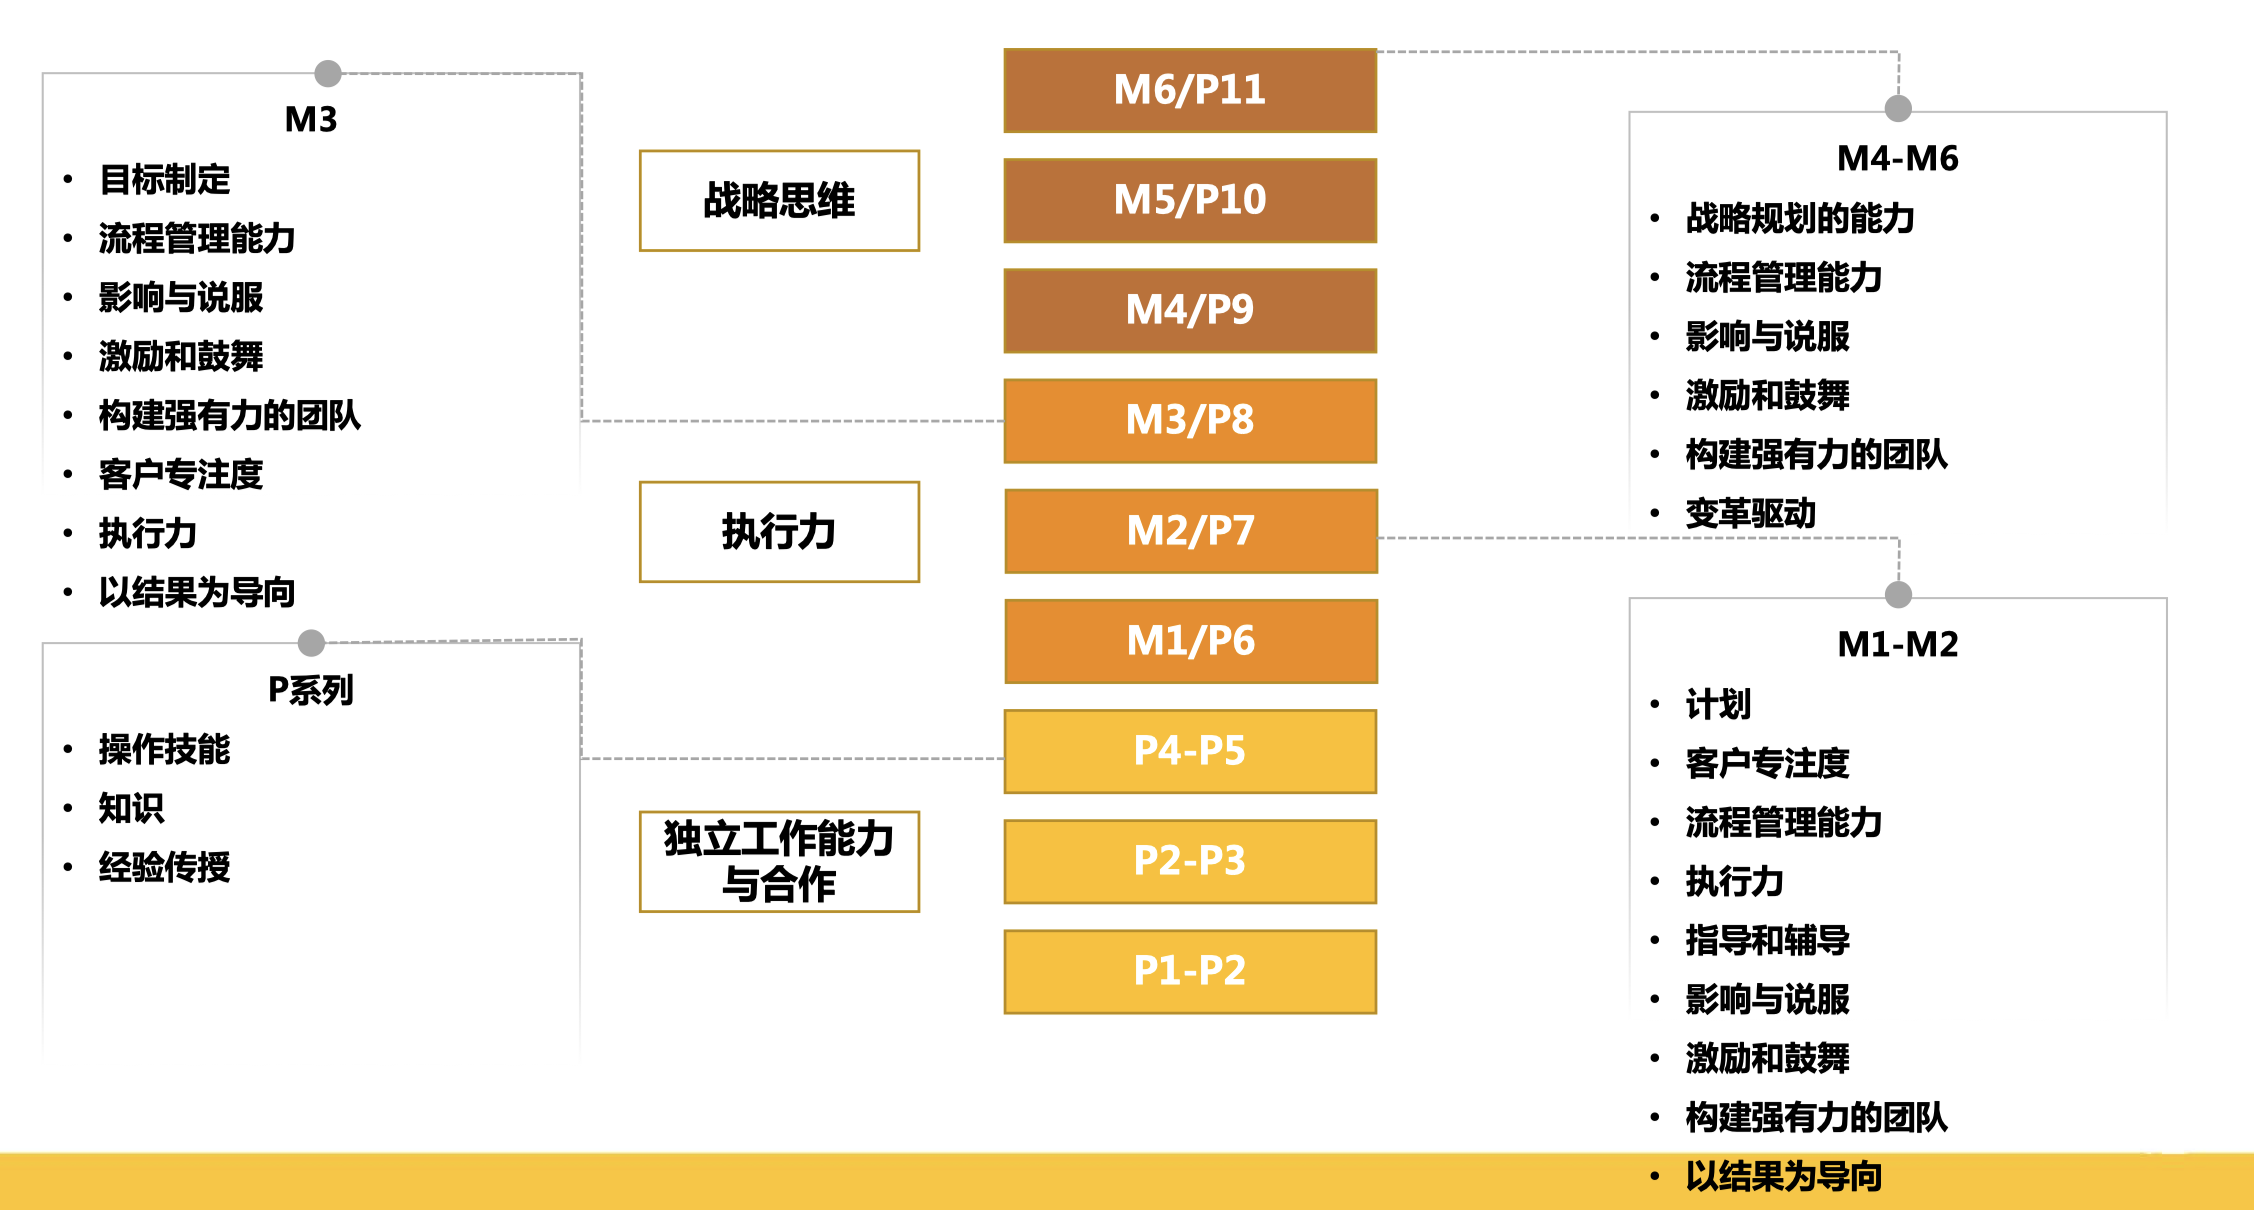
\includegraphics[width=1\textwidth]{fig/Ali_Performance_15.png}
\end{figure}



%\printbibliography
\bibliography{../ref}
\bibliographystyle{IEEEtran}
\end{document}
